\documentclass[11pt]{article}
\usepackage[margin=1in]{geometry} % Adjust margins as needed
%!TEX root = ./main_source.texx
\UseRawInputEncoding
\usepackage{hyperref}
% For authors with multiple institutions
\usepackage[affil-sl]{authblk}
% For line-numbers in my document
\usepackage{lineno}

% Redefine the cite color to your preferred color

\usepackage[utf8]{inputenc}
\usepackage[T1]{fontenc}
\usepackage{anyfontsize}
\usepackage{lipsum} % For dummy text
\usepackage{microtype} % Improved font rendering
\usepackage{titlesec} % Customize section titles
\usepackage{graphicx} % For including images
\usepackage{bm}
\usepackage{svg}
\usepackage{xcolor}
% \usepackage{ulem}
\usepackage{bbm}
\usepackage{xspace}
\usepackage{tabularx}
\usepackage{stmaryrd}
\SetSymbolFont{stmry}{bold}{U}{stmry}{m}{n}
\usepackage{bbm}
\usepackage{url}            % simple URL typesetting
\usepackage{booktabs}       % professional-quality tables
\usepackage{amsfonts}       % blackboard math symbols
\usepackage{nicefrac}       % compact symbols for 1/2, etc.
\usepackage{microtype}      % microtypography
\usepackage{amsmath,amsthm}
\usepackage{tikz}
\usepackage[most]{tcolorbox}

\usepackage{natbib}
% \bibliographystyle{dinat}
% \setcitestyle{authoryear, open={[},close={]}} %Citation-related commands

%\usepackage{amssymb}
\let\Bbbk\relax
\usepackage{newtxmath}
\usepackage{letltxmacro}
\usepackage{bm}

\usepackage{soul}
\usepackage[linesnumbered,ruled,vlined]{algorithm2e}
\usepackage[compatible]{algpseudocode} 
\usepackage{bbm}
\usepackage{svg}
\usepackage{xcolor}
\usepackage{xspace}
\usepackage{stmaryrd}
\usepackage{bbm}
\usepackage{url}            % simple URL typesetting
\usepackage{booktabs}       % professional-quality tables
\usepackage{nicefrac}       % compact symbols for 1/2, etc.
\usepackage{microtype}      % microtypography
\usepackage{letltxmacro}
\usepackage{bm}
\usepackage{caption}
\usepackage{subcaption}
\usepackage{soul}
\usepackage[linesnumbered,ruled,vlined]{algorithm2e}
\usepackage[compatible]{algpseudocode} 
% \usepackage{pgfplots}
\usepackage{doi}
\usepackage{fancyvrb,cprotect}
\usepackage{centernot}
\usepackage{fancyhdr}
\graphicspath{ {assets/} }


\definecolor{amber}{rgb}{1.0, 0.49, 0.0}
\definecolor{cadmiumgreen}{rgb}{0.0, 0.42, 0.24}
\definecolor{darkcyan}{rgb}{0.0, 0.55, 0.55}
\definecolor{darkcoral}{rgb}{0.8, 0.36, 0.27}
\definecolor{azure}{rgb}{0.0, 0.5, 1.0}
\definecolor{bittersweet}{rgb}{1.0, 0.44, 0.37}
\definecolor{razzmatazz}{rgb}{0.89, 0.15, 0.42}
\definecolor{ballblue}{rgb}{0.13, 0.67, 0.8}
\definecolor{purple}{rgb}{0.2, 0.2, 0.6}
\definecolor{egyptianblue}{rgb}{0.06, 0.2, 0.65}
\definecolor{darkslategray}{rgb}{0.0, 0.29, 0.29}
\definecolor{bananayellow}{rgb}{1.0, 0.88, 0.21}
\definecolor{blue-violet}{rgb}{0.54, 0.17, 0.89}
\definecolor{carminepink}{HTML}{EF58A0}
\definecolor{titlecolor}{RGB}{0,74,147}
\definecolor{sectioncolor}{RGB}{0,129,255}
\definecolor{subsectioncolor}{RGB}{0,129,255}
\definecolor{definitioncolor}{rgb}{0.89, 0.0, 0.13}
\usepackage{hyperref} 

\hypersetup{
    colorlinks=true,
    linkcolor=cadmiumgreen,
    citecolor=carminepink, % Set color for citation links
    urlcolor=titlecolor % Set color for URL links
}

\newcommand{\highlight}[1]{\color{razzmatazz} #1 \color{black}}
\newcommand{\ari}[1]{\textcolor{purple}{\textbf{[Ari]:} #1}}
\newcommand{\attentionC}[1]{\textcolor{orange}{\textbf{Attention Cl\'ement:}}\textcolor{blue}{\quad#1}}
\newcommand{\ykResolved}[1]{\textcolor{orange}{\textbf[YK] \sout{#1}}}
\newcommand{\CC}[1]{\textcolor{carminepink}{\textbf[CC] #1}}
\newcommand{\CCResolved}[1]{\textcolor{carminepink}{\textbf[CC] \sout{#1}}}
\usepackage{cleveref}       % smart cross-referencing


\usepackage{framed}
\usepackage{rotating}

\usepackage[colorinlistoftodos]{todonotes}
% todo leftbar
% \newenvironment{todo}{ %
% \def\FrameCommand{\hspace{-2em}%
% \begin{sideways}%
% \textcolor{red}{\textsf{\small TODO}}%
% \end{sideways}%
% \hspace{0.5em}\textcolor{red}{\vrule width 0.5pt} \hspace{0.5em}}\MakeFramed {\advance\hsize-\width \FrameRestore}}
% {\endMakeFramed}



%\newcommand{\email}[1]{\texttt{#1}}
\usepackage{accents}
\usepackage{calc}
%%%%%%%%%%%%%%%%%%%%%%%%%%%%%%
% Theorem
% Define a new theorem style
\newtheoremstyle{theoremstyle}
  {\topsep} % Space above
  {\topsep} % Space below
  {} % Body font
  {} % Indent amount
  {\bfseries\color{black}} % Theorem head font
  {} % Punctuation after theorem head
  {.5em} % Space after theorem head
  {\thmname{#1}~\thmnumber{#2}:~\textcolor{carminepink}{\thmnote{[#3]}}} % Theorem head spec (can be left empty, meaning ‘normal’)

% Define mdframed settings for the lemma box
\mdfdefinestyle{theoremframe}{
  linecolor=theoremcolor!80,
  linewidth=2pt,
  backgroundcolor=theoremcolor!15,
  roundcorner=5pt,
  nobreak=true,
  topline=false,
  bottomline=false,
  rightline=false,
}
% Apply the custom theorem style
\theoremstyle{theoremstyle}
% Define a theorem environment
\newtheorem{theorem}{Theorem}[section]
% Automatically surround lemma with mdframed
\surroundwithmdframed[style=theoremframe]{theorem}


%%%%%%%%%%%%%%%%%%%%%%%%%%%%%%
% Remark
\newtheoremstyle{remarkstyle}
  {\topsep} % Space above
  {\topsep} % Space below
  {} % Body font
  {} % Indent amount
  {\bfseries\color{black}} % Theorem head font
  {} % Punctuation after theorem head
  {0.5em} % Space after theorem head
  {} % Theorem head spec (can be left empty, meaning ‘normal’)

% Define mdframed settings for the lemma box
\mdfdefinestyle{remarkframe}{
  linecolor=fuyu-gaki!80,
  linewidth=2pt,
  backgroundcolor=fuyu-gaki!15,
  roundcorner=5pt,
  nobreak=true,
  topline=false,
  bottomline=false,
  rightline=false,
}
% Apply the custom theorem style
\theoremstyle{remarkstyle}
\newtheorem{remark}{Remark}
\surroundwithmdframed[style=remarkframe]{remark}
\newtheorem{corollary}{Corollary}
\surroundwithmdframed[style=remarkframe]{corollary}

\newtheoremstyle{definitionstyle}
  {\topsep} % Space above
  {\topsep} % Space below
  {} % Body font
  {} % Indent amount
  {\bfseries\color{black}} % Theorem head font
  {} % Punctuation after theorem head
  {.5em} % Space after theorem head
  {\thmname{#1}~\thmnumber{#2}:~\textcolor{carminepink}{\thmnote{[#3]}}} % Theorem head spec (can be left empty, meaning ‘normal’)

% Define mdframed settings for the lemma box
\mdfdefinestyle{definitionframe}{
  linecolor=definitioncolor!80,
  linewidth=2pt,
  backgroundcolor=definitioncolor!45,
  roundcorner=5pt,
  nobreak=true,
  topline=false,
  bottomline=false,
  rightline=false,
}
\theoremstyle{definitionstyle}
\newtheorem{definition}[theorem]{Definition}
\surroundwithmdframed[style=definitionframe]{definition}

%%%%%%%%%%%%%%%%%%%%%%%%%%%%%%
% Lemma
% Define a new theorem style
\newtheoremstyle{lemmastyle}
  {\topsep} % Space above
  {\topsep} % Space below
  {} % Body font
  {} % Indent amount
  {\bfseries\color{black}} % Theorem head font
  {} % Punctuation after theorem head
  {.5em} % Space after theorem head
  {\thmname{#1}~\thmnumber{#2}:~\textcolor{carminepink}{\thmnote{[#3]}}} % Theorem head spec (can be left empty, meaning ‘normal’)

% Define mdframed settings for the lemma box
\mdfdefinestyle{lemmaframe}{
  linecolor=theoremcolor!80,
  linewidth=2pt,
  backgroundcolor=theoremcolor!05,
  roundcorner=5pt,
  nobreak=true,
  topline=false,
  bottomline=false,
  rightline=false,
}
% Apply the custom theorem style
\theoremstyle{lemmastyle}
\newtheorem{lemma}[theorem]{Lemma}
% Automatically surround lemma with mdframed
\surroundwithmdframed[style=lemmaframe]{lemma}
\newtheorem{claim}[theorem]{Claim}
% Automatically surround lemma with mdframed
\surroundwithmdframed[style=definitionframe]{claim}

% Define custom environments for Question and Open Problem
% \newenvironment{question}
%   {\reversemarginpar
%    \marginnote{\textbf{\textcolor{fuyu-gaki}{Question:}}}}
%  {}

\newtcolorbox[auto counter, number within=section]{problem}[2][]{colframe=fuyu-gaki, colback=mizu!10, coltitle=white, title={Problem }, sharp corners, boxrule=0.8mm, width=0.99\textwidth, boxsep=2mm, left=3mm, right=3mm, top=2mm, bottom=2mm, breakable}



%%%%%%%%%%%%%%%%%%%%%%%%%%%%%%
\newcommand{\goal}[1]{
\begin{tcolorbox}[colframe=red!50!black, colback=white!95!black,title=Goal]
#1
\end{tcolorbox}    
}


% Common stuff that show up in nearly all writeups
\newcommand{\Def}{=}
\makeatletter
\newcommand{\smalldollar}{\mathrel{\mathpalette\small@dollar\relax}}
\newcommand{\small@dollar}[2]{%
  \vcenter{\hbox{%
    $#1\textnormal{\fontsize{0.7\dimexpr\f@size pt}{0}\selectfont\$}$%
  }}%
}
\makeatother
\renewcommand{\emph}[1]{\textit{#1}}
\newcommand\Bigger[2][7]{\left#2\rule{0mm}{#1truemm}\right.}
\renewcommand{\vec}[1]{\mathbf{#1}}
\newcommand{\TODO}{\textcolor{orange}{??TODO??}}
\renewcommand{\epsilon}{\varepsilon}
\newcommand{\Set}[1]{\left\{ #1\right\}}
\newcommand{\RCloseLOpenInterval}[2]{}
\newcommand{\LCloseROpenInterval}[2]{\left[#1, #2\right)}
\newcommand{\Interval}[2]{\left[\right]}
\newcommand{\OpenInterval}[2]{\left(\right)}
\newcommand{\DistSet}[1]{\Delta(#1)}
\newcommand{\Dist}{\mathcal{D}}
\newcommand{\leftarrowS}{\leftarrow\joinrel\smalldollar}
\newcommand{\rightarrowS}{\smalldollar\joinrel\rightarrow}
\newcommand{\samples}{\highlight{\leftarrowS}}
\newcommand{\negl}{\mathtt{negl}}
\newcommand{\Indicator}[1]{\mathbbm{1}\left\{#1\right\}}
\newcommand{\Eps}{\textcolor{red}{\varepsilon}}
\newcommand{\EpsLower}{\textcolor{shin-kai}{\varepsilon'}}
\newcommand{\EpsUpper}{\textcolor{shin-kai}{\varepsilon}}
\renewcommand{\tilde}[1]{\widetilde{#1}}
\newcommand{\bit}{\{0,1\}}
\newcommand{\poly}{\mathsf{poly}}
\newcommand{\Naturals}{\mathbb{N}}
\newcommand{\Integers}{\mathbb{Z}}
\newcommand{\Reals}{\mathbb{R}}
\newcommand{\Field}{\mathbb{F}}
\newcommand{\BigO}[1]{O\left(#1\right)}
\newcommand{\BigOTilde}[1]{\tilde{O}\left(#1\right)}
\newcommand{\SmallO}[1]{o\left(#1\right)}
\newcommand{\BigOmega}[1]{\Omega\left(#1\right)}
\newcommand{\SmallOmega}[1]{\omega\left(#1\right)}
\newcommand{\Mean}[2]{\mathbb{E}_{#1}\left[#2\right]}
\newcommand{\Prob}[1]{\Pr\left[#1 \right]}
\newcommand{\PProb}[2]{\Pr_{#2}\left[#1 \right]}
\newcommand{\True}{\texttt{True}}
\newcommand{\False}{\texttt{False}}


% Complexity classes 
\newcommand{\BPP}{\mathsf{BPP}}
\renewcommand{\P}{\mathsf{P}}
\newcommand{\NP}{\mathsf{NP}}
\newcommand{\CoNP}{\mathsf{coNP}}

% Paper specific + Proof Complexity Macros
\newcommand{\PropFormula}{\Phi}
\newcommand{\Proof}{\pi}
\newcommand{\Size}[1]{|#1|}
\newcommand{\Card}[1]{\text{Card}(#1)}
\newcommand{\Axioms}{\mathcal{Q}}
\newcommand{\axiom}{q}
\newcommand{\PM}[1]{\text{PM}(#1)}
\newcommand{\RemGraph}{G'}
\newcommand{\BadSet}{\textcolor{blue}{\hat{S}}}
\newcommand{\ari}[1]{\textcolor{kon-peki}{Ari: }#1}
\newcommand{\highlight}[1]{\textcolor{yama-budo}{#1}}
\newcommand{\red}[1]{\textcolor{fuyu-gaki}{#1}}
\newcommand{\green}[1]{\textcolor{shin-ryoku}{#1}}
\newcommand{\RedNodes}[1]{\red{\text{Red}}(#1)}
\newcommand{\GreenNodes}[1]{\green{\text{Green}}(#1)}
\newcommand{\GreenB}{\green{B}}
\newcommand{\RedA}{\red{A}}
\newcommand{\BipartiteG}{G_{\GreenB \cup \GreenB}}
\newcommand{\SizeRemGraph}{n'}

% Graph Commands
\newcommand{\Graph}{G}
\newcommand{\Vertices}[1]{\mathsf{V}(#1)}
\newcommand{\Edges}[1]{\mathsf{E}(#1)}
\newcommand{\CutEdges}[3]{e(#1 \leftrightarrow #2; #3)}
\newcommand{\IncidentEdges}[1]{\mathsf{E}(\rightarrow #1)}
\newcommand{\CutEdgesSet}[3]{\mathsf{E}(#1 \leftrightarrow #2; #3)}
\newcommand{\OddComponents}[1]{q(#1)}
\newcommand{\degree}[2]{\mathsf{deg}_{#1}(#2)} 
\newcommand{\MaxDegree}[1]{\Delta_{#1}}
\newcommand{\Neighbourhood}[2]{\Gamma_{#1}\left(#2\right)}
\newcommand{\Family}[1]{\textcolor{purple}{\mathcal{#1}}}
\newcommand{\SafeStates}{\Family{S}}
\newcommand{\HardInstance}{H}
\newcommand{\Embedding}[1]{\Psi\left(#1\right)}
\newcommand{\Path}[2]{\mathsf{P}_{#1 \rightsquigarrow #2
}}
\newcommand{\PathSize}{\textcolor{red}{l}}
\newcommand{\GlobalEdgeSet}{\textcolor{orange}{\mathcal{E}}}
\newcommand{\Degree}[1]{\text{Deg}\left(#1\right)}
\newcommand{\PerfectMatching}[1]{\mathsf{PM}\left(#1\right)}
\newcommand{\Complement}[1]{\overline{#1}}
\newcommand{\EdgeConnectivity}[1]{\kappa'(#1)}
\newcommand{\PC}{\vdash_{\texttt{PC}_F}}
\newcommand{\SOS}{\vdash_{\texttt{SOS}}}
\newcommand{\en}{\textcolor{ballblue}{n}}
\newcommand{\dee}{\textcolor{cadmiumgreen}{d}}
\newcommand{\eigen}{\textcolor{red}{\lambda}}
\newcommand{\EnDeeLambda}{(n, d, \lambda)}
\newcommand{\Subdivision}[2]{{#1}^{#2}}
\newcommand{\MinimalDegree}[1]{\delta_{#1}}
\newcommand{\dbtilde}[1]{\tilde{\raisebox{0pt}[0.85\height]{$\tilde{#1}$}}}
\newcommand{\na}{\green{n_B}}
\newcommand{\EdgesShort}{E}
\newcommand{\ExpansionFactor}[1]{\lambda(#1)}
\newcommand{\EmbeddingFunc}{\Psi}



 %These are generic commands (Might move them to %base template)is

% Intro
%\newcommand{\P}{\mathsf{P}}
%\newcommand{\NP}{\mathsf{NP}}

\synctex=1
% Title
\title{Sum of Squares Refutations of Perfect Matchings In Expander Graphs Is Hard}

%\sqrt{\nicefrac{d}{2}\log (2/\delta)} ; this is the error term

% \author{}
\author[1]{Ari Biswas}
\author[2]{Rajko Nenadov}
\affil[1]{\small University Of Warwick, United Kingdom}
\affil[2]{\small University Of Auckland, New Zealand}

\date{}
% \linenumbers
\begin{document}

\maketitle
\begin{abstract}
\ari{Under heavy re-factoring. Do not look yet!}
\end{abstract}

\section{Introduction}


\begin{figure}
	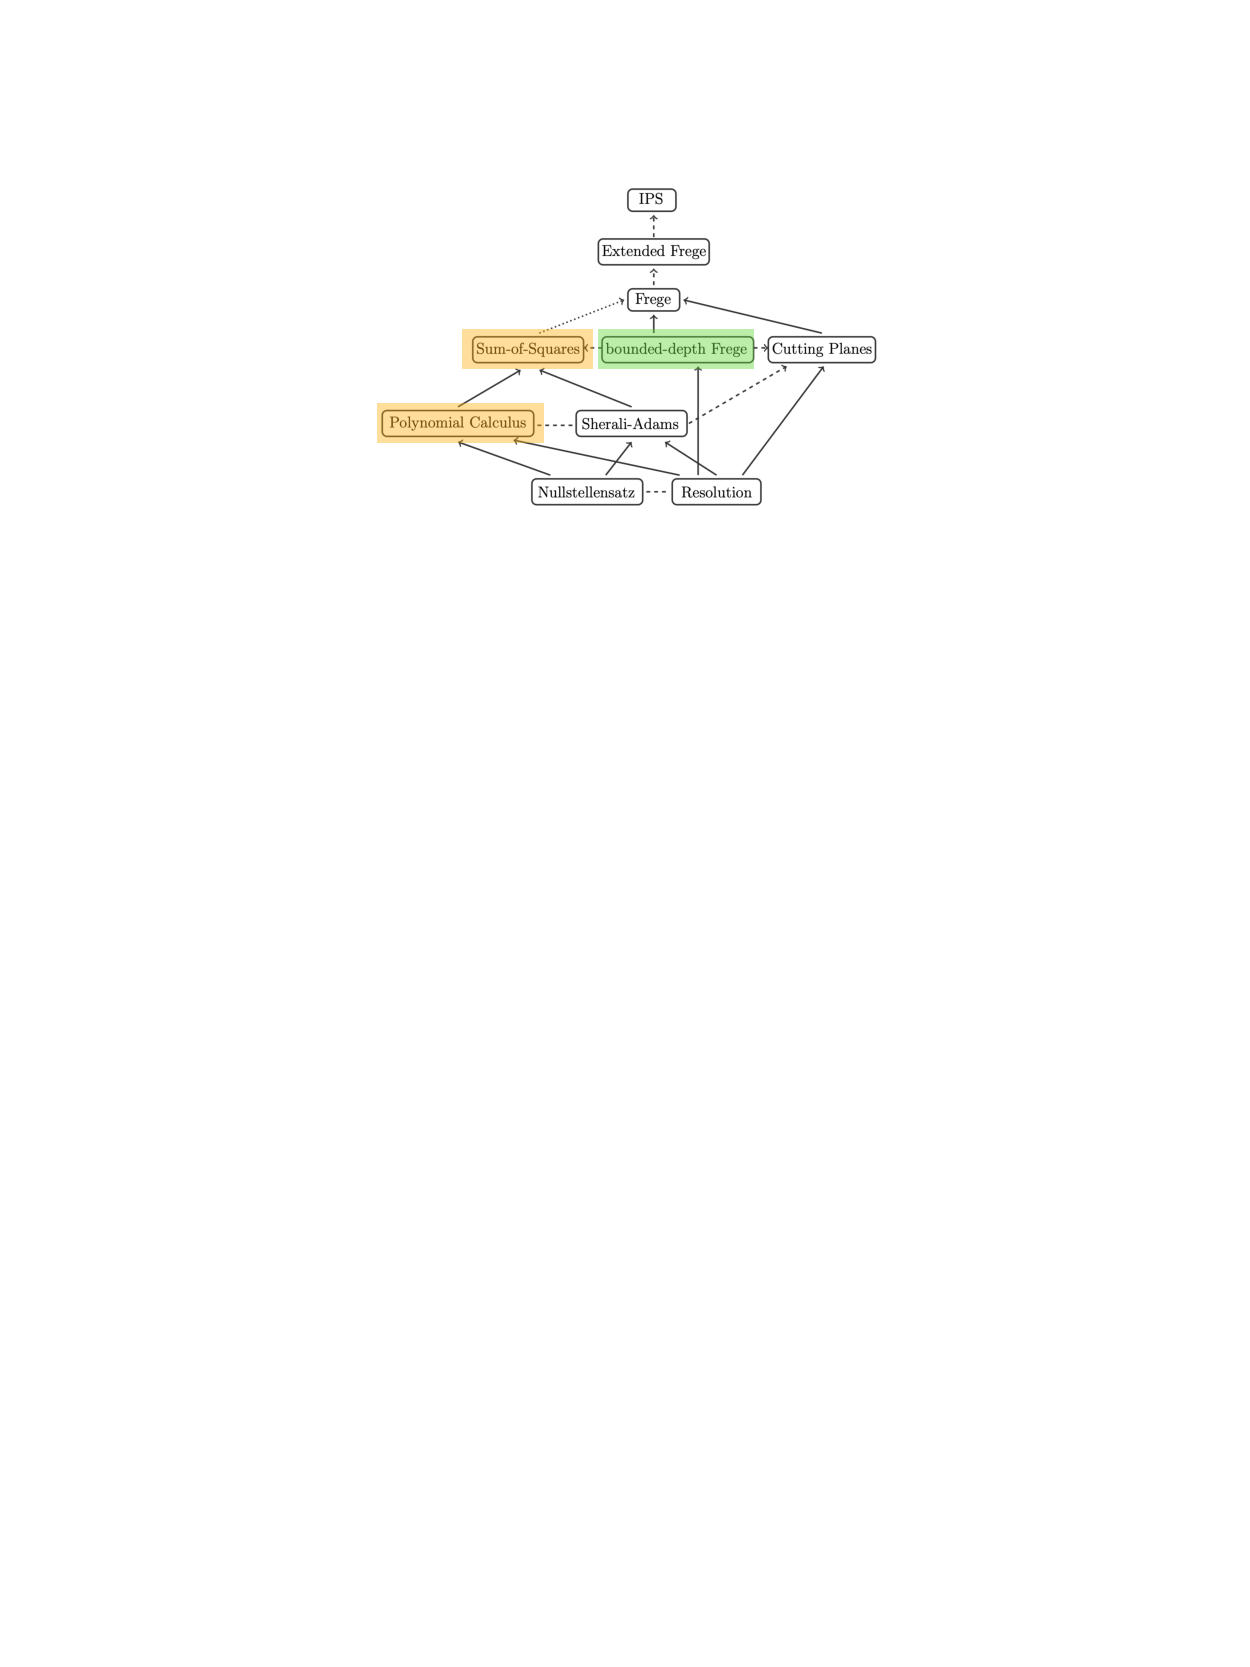
\includegraphics{assets/proof-system-relationships.pdf}
	\caption{The figure above (sourced from \citep[Page 10]{ProofComplexityLecNotes}) depicts proof systems commonly studied by the community and how they relate to each other.}
	\label{fig:example-proof-systems}
\end{figure}


Perhaps the most fundamental problem in computation is to provide an answer to the question: ``\textit{Given a true statement $A$, what is the shortest proof of the claim that $A$ is true?}''
In trying to answer this question, \citet{cook1979relative} observed that we must first describe what constitutes a valid proof?
That is, we must describe the language in which the proof is written, and the rules for checking it.
Each set of rules for writing and checking a proof defines a proof system.
Therefore, a precise restatement of the question above is the following:  ``\textit{Given a true statement $A$ and a proof system $S$, what is the length of the shortest proof $\Proof \in S$ that proves $A$?}''
If we could show that there exists a proof system $S$, such that for any true statement $A$, the length of the shortest proof in $S$ is upper bounded by some polynomial in the length of $A$, it would imply that $\CoNP = \NP$, which would further imply that $\P = \NP$.
Conversely, if we could show large proof size lower bounds for $A$ in all proof systems, it would lead to a formal proof of the widely believed conjecture that $\P \neq \NP$.
Unfortunately, we currently do not possess the tools to show lower such bounds for \emph{arbitrary} proof systems.
Thus, as an intermediate step towards making partial progress towards the grand problem, the research community has invested a significant amount of time and energy in proving size lower bounds for certain specific proof systems \citep{blake1937canonical,razborov1998lower, impagliazzo1999lower, alekhnovich2001lower, buss1999linear}.
\todo{Change this figure to the one in pitassi flemming which includes the relevant proof systems for us} Figure \ref{fig:example-proof-systems} lists some these proof systems and describes the relationships between them.
Proof systems listed at the top of Figure \ref{fig:example-proof-systems} are more expressive\footnote{Expressiveness is formalised by the notion of $p$-simulation, and we refer the reader to \citep[Definition 1.6]{ProofComplexityLecNotes} for more details.}, and lower bounds for such proof systems subsume claims about the complexity of proofs lower in the figure.
We refer the reader to \citep{krajicek2019proof, ProofComplexityLecNotesPaul} for more details on the definitions of the various proof systems.\par
%One example of a simple proof system is that of truth tables i.e. given a propositional formula $\PropFormula$ that is a tautology, a valid proof is simply the truth table for the formula.
%A formula on $n$ variables requires truth tables with size $2^n$, and it is easy to see that we cannot use shorter proofs.
%Although simple, truth tables are quite inefficient\footnote{A proof system $A$ is more inefficient than a proof system $B$ if proofs of the same claim are longer in $A$ compared to $B$.} proof systems, and there exists proof systems that can have much shorter proofs for certain problems than possible with truth tables.

In this work, we focus on the algebraic and semi-algebraic proof system of polynomial calculus (PC) \citep{alekhnovich2004pseudorandom} and sum of squares (SOS) proof system \citep{parrilo2000structured, boazCourse}.
In proof systems like PC and SOS, instead of a propositional formula over $n$ variables, we are given a set $\Axioms =\{\axiom_i(\vec{x}) \text{ } |\text{ } i \in [m] \}$ of $m$ polynomial equations\footnote{Semi-algebraic proof systems also allow for inequalities but we will not deal with inequality constraints in this paper.} over $n$ variables $\vec{x} = \{x_1, \dots, x_n\}$ as the problem instance.
In PC, the polynomial coefficients can be over \emph{any} field $\Field$, and in SOS, the polynomial coefficients must be over the reals.
We say a proof $\Proof$ is a refutation of $\Axioms$, if it is a proof of the claim (in the specified language) that there exists no assignment of $\vec{x} \in \Field^n$ that satisfies \emph{all} the polynomial equations in $\Axioms$. 
In PC and SOS, the proof $\Proof$ is itself expressed as a sequence of polynomials, and 
the size/complexity of the proof is measured by the maximum of degree of the proof polynomials that refutes $Q$ (see Section \ref{sec:proof-system-prelims} for more formal details).
We denote the minimum degree of a proof that refutes $\Axioms$ with $\Degree{\Axioms \PC \bot}$ and $\Degree{Q \SOS \bot}$ for PC and SOS respectively, and the main goal of the area is to study how large is the degree of proofs for refuting a given set of axioms $\Axioms$.
Although algebraic by definition, one can use these proof systems to refute properties of combinatorial objects like graphs, and it even serves as a proof system for UNSAT.\par
In this paper we consider refutations of the perfect matching principle.
More specifically, given an undirected graph $G=(V,E)$, and a vector $\vec{b} = (b_1, \dots, b_{|V|})  \in \Field^{\Size{V}}$, we define $\Card{G, \vec{b}}$ as the following set of polynomial constraints over variables $x_1, \dots, x_{|E|} \in \Field^{\Size{E}}$

\[
        \Card{G, \vec{b}}=
        \Bigger[10]\{\begin{array}{@{}cl}
                x_{\highlight{e}}(1 - x_{\highlight{e}}) = 0 & \text{ for every $\highlight{e} \in E$}\\[3mm]
                \underset{u \text{ is a neighbour of }\highlight{v}}{\sum x_{(u,\highlight{v})}}= b_{\highlight{v}} & \text{ for every $\highlight{v} \in V$} \\[3mm]
        \end{array}
\]

For every $e \in E$, if the polynomial equation $x_e(1 - x_e) = 0$ were to be satisfied, then it restricts the domain of the above variables to bits i.e. $x_e \in \bit$ for all $e \in E$.
Note if there was an assignment of variables in $\vec{x} \in \bit^{|E|}$ that satisfied all the equations in $\Card{G, 1^{|V|}}$, it would imply that the graph $G$ has a perfect matching (given by the edges corresponding to variables with assignment 1).  
When $\vec{b} = 1^{|V|}$, as short hand we denote $\Card{G, \vec{b}}$ as $\PM{G}$.
When $|V|$ is odd, we know that any graph $G$ cannot have a perfect matching.
In other words, $\Card{G, 1^{|V|}}$ cannot be satisfied.
In this work we are interested in the complexity refutations for $\PM{G}$  when $|V|$ is odd in PC and SoS proof systems.
With no further constraints on $G$, generic lower bounds for these refutations in PC or SOS proof systems are not known.
In their recent manuscript \citep[Open Problem 7.7]{buss2021proof}, Buss and Nordstr{\"o}m asked ``\textit{Are even colouring formulas over expander graphs hard for
polynomial calculus over fields of characteristic distinct from 2 ?}''
The even colouring formula is a special case of $\Card{G, \vec{b}}$, where each coordinate  $\vec{b}$ is $\degree{G}{v}/2$ for $v \in V$.
Therefore, their open question can be reformulated as the following question.

\begin{problem}

Do refutations for $\Card{G, \vec{b}}$ for
polynomial calculus over fields of characteristic $\neq 2$ have large size, when $G$ is an expander graph? \citep[Open Problem 7.7]{buss2021proof}

\end{problem}

\citet{Austrin_2022} made partial progress on the above problem by showing that the perfect matching principle requires large size on \emph{random $d$-regular graphs} (where $d \in \BigO{1}$) in the Sum-of-Squares and Polynomial Calculus proof systems \emph{on average}.
More formally, they show that 

\begin{theorem}\label{thm:prev-thm}
There is a constant $d_0 \in \Naturals$ such that for all $d \geq d_0$, and $\vec{b} \in [d]^{\Size{V}}$, the following holds \emph{asymptotically almost surely} over a random $d$-regular graph $G=(V,E)$ on $n$ vertices:
\begin{enumerate}
    \item{ $\Degree{\Card{G, \vec{b}} \PC \bot} = \BigOmega{\frac{n}{\log n}}$} 
    \item{$\Degree{\Card{G, \vec{b}} \SOS \bot} = \BigOmega{\frac{n}{\log n}}$}
\end{enumerate}
\end{theorem}

Given a random $d$-regular graph $G\samples \mathcal{G}(n, d)$ on $n$ vertices (where $n$ is odd), the authors start with a worst case hard graph $H$ described by \citet{buss1999linear}.
%Such a graph is known to have $\Degree{\PerfectMatching{G} \PC \bot} = \BigOmega{\Size{V(H)}}$ (see \citep[Appendix A]{Austrin_2022} for details about how $H$ is constructed and \citet{buss1999linear} for hardness proof).
Their average case hardness result then comes by \emph{embedding} $H$ into $G$ in such a way that that the hardness of $H$ is transferred to $G$.
Thus, the main contribution of \citet{Austrin_2022} is a novel embedding theorem that embeds $H$ as a topological minor into $G $ where edges in $H$ are mapped to odd length paths in the embedding.
A distinctive feature of their result is that as the embedding relies on randomness used to sample the regular graph, and thus they only provide average case lower bounds.
These techniques do not apply when the host graph $G$ is constructed deterministically, as in the case of the many known deterministic constructions of expander graphs.

\todo{Needs an edit. Describe how they depend on randomness better, now that i understand it better.}
\paragraph{Our Contribution} In this work, we directly answer Buss and Nordstr{\"o}m's question by showing hardness results that do \emph{not} rely on randomness, and therefore allowing us to prove worst case lower bounds for refuting perfect matchings in any large enough expander graph with an odd number of vertices.
It should be noted that as an expander graph is \emph{also} a random graph with high probability, our result subsumes the result of \citet{Austrin_2022}.
A second defining feature of our contribution is the qualitative simplicity of the hardness result.
To show their hardness results, Austrin and Risse embed the hard instance $H$ constructed by \citet{buss1999linear} in a random $d$ regular graph $G$.
To do this, they first show a partition lemma that partitions the vertices of $G$ into two sets $T$ and $\Vertices{G} \setminus T$, such that the partition satisfies two properties.
The first property requires that for any odd sized subset $U \subseteq T$, $\Vertices{G} \setminus U$ has a perfect matching.
This property is used to inherit the hardness of $H$ into $G$ (ensuring that there is no shorter refutation using parts of $G$ not used for the embedding).
%In contrast, we show a much simpler way to inherit the hardness of $H$ into any pseudo random graph (even deterministic constructions) via a simple application of the Tutte criterion (Lemma \ref{lemma:tutte-criterion}). 
The second property, requires the induced subgraph $G[T]$ contains a constant degree $\alpha$ vertex expander such that the maximal degree of $H$ is $\MaxDegree{H} \ll \alpha^2 \degree{}{G}$.
The primary reason the authors require the second property, is to be able to use a result by \citet{krivelevich2019completeminorsgraphssparse}, which allows us to embed any graph $H$ into a host graph $\tilde{G}$ as a minor, if $\tilde{G}$ is a vertex expander with the above properties.
%They describe an iterative algorithm for  embedding the vertices of $H$ into $\tilde{G}$ one while keeping track of the unused vertices of $\tilde{G}$, and discarding bad vertices that lead to bad embeddings and restarting the process of finding good vertices again \ari{Rajko can likely provide a better summary of his own work}.
However, Austrin and Risse cannot directly use the result in \citep{krivelevich2019completeminorsgraphssparse} as they need to embed $H$ as a \emph{topological} minor in a $d$-random graph $G$ instead of embedding it as an ordinary minor.
Thus, their main technical contribution is a modification of \citet{krivelevich2019completeminorsgraphssparse} to allow for topological embeddings.
To embed $H$ as a topological minor, Austrin and Risse need to find vertex disjoint odd length paths in $G$ for edges in $H$.
Therefore they map vertices of $H$ to ``star-like'' subgraphs in $G$, which allows the central vertex of the star to be connected to many vertex disjoint paths without incurring collisions.
Formally proving the result requires a fairly involved set of tools from spectral graph theory, and forms the basis of their main technical contribution.
In this work, we show a direct way to embed $H$ into any expander graph inspired by ideas from the theory of wide sense non blocking networks \citep{feldman1988wide}.
The only spectral graph theory we require is the expander mixing lemma (Lemma \ref{lemma:expanders-mixing-lemma}).
Furthermore, showing that the rest of graph contains a perfect matching, and therefore the hardness of $H$ is transferred, can be shown by a simple application of the Tutte criterion (Lemma \ref{lemma:tutte-criterion}).
In summary, we show \emph{stronger} lower bounds for a \emph{larger} set of objects using \emph{simpler} proof techniques.
Our main result is stated below.

\begin{theorem}[Main Theorem]\label{thm:main-thm}

There is constants $n_0, d_0 \in \Naturals$ such that for all $d \geq d_0$, the following holds  for \emph{any} $(n, d, \lambda)$-graph $G$ on $n \geq n_0$ vertices, where $n$ is odd and $\lambda < \highlight{TODO}$:
\begin{enumerate}
    \item{ $\Degree{\PerfectMatching{G} \PC \bot} = \BigOmega{\frac{n}{\log n}}$} 
    \item{$\Degree{\PerfectMatching{G} \SOS \bot} = \BigOmega{\frac{n}{\log n}}$}
\end{enumerate}

\end{theorem}

The rest of the document as is structured as follows. In section \ref{sec:prelims} we describe the requisite background from graph theory and proof complexity required to describe and derive the Theorem \ref{thm:main-thm}.
In Section \ref{sec:embed-machinery}, we review definitions and results from the theory of wide-sense nonblocking networks, which aid us in the construction of our main embedding theorem.
In Section \ref{sec:main-proof}, we provide the full proof of the main result and in Section \ref{sec:related-work} we describe related results in proof complexity lower bounds using embedding techniques.
Finally, in Section \ref{sec:conclusion} we conclude with some open problems that we could not resolve in this work.


\section{Preliminaries}
\label{sec:prelims}

We review some basic tooling used for proving existence of objects using the probabilistic method.




\subsection{Graph Theory Preliminaries}
\label{sec:graph-theory-prelims}

For a graph $\Graph$, we use $\Vertices{\Graph}$ and $\Edges{\Graph}$ to denote the vertices and edges of $\Graph$. 
For any $E' \subseteq \Edges{\Graph}$ and a vertex $v \in \Vertices{\Graph}$, we use $\Neighbourhood{E'}{v} = \{ u \in \Vertices{\Graph} : (u,v) \in E' \}$ to denote the neighbourhood of $v$ with respect to $E'$, and $\degree{E'}{v}$ to denote the number of vertices adjacent to $v$ via edges in $E'$.
We assume the reader is familiar with standard graph theory definitions of subgraphs, minors, subdivisions and  topological minors.
We refer the reader to \citep{bollobas2012graph} for a detailed introduction to these concepts.
Next we define pseudorandom graphs or expander graphs. 
Throughout this document, it suffices to treat $d$ as a small constant.

\begin{definition}[$\EnDeeLambda$ pseudorandom graphs]\label{def:expander-graphs}
Let $G$ be a $d$-regular graph on $n$ vertices, and, let $\lambda_1 \geq \lambda_2, \dots, \geq \lambda_n$ denote eigenvalues of the adjacency matrix of $G$.
We say $G$ is an $\EnDeeLambda$-graph if $\ExpansionFactor{\Graph} \Def \underset{{\{2, \dots, n\}}}{\max}|\lambda_i| \leq \lambda$.
\end{definition}


\begin{lemma}[Expander Mixing Lemma]\label{lemma:expanders-mixing-lemma}
  Given an $\EnDeeLambda$ graph $G$ for any $S, T \subseteq \Vertices{G}$ we have
\begin{align*}
  \CutEdges{S}{T}{\Edges{G}} &\geq \frac{d\Size{S}\Size{T}}{n} - \lambda\sqrt{\Size{S}\Size{T} (1 - \frac{\Size{S}}{n}) (1 - \frac{\Size{T}}{n})   }	\\
  &\geq \frac{d\Size{S}\Size{T}}{n} - \lambda\sqrt{\Size{S}\Size{T} }
\end{align*}
  
\end{lemma}





\subsection{Proof Complexity Preliminaries}
\label{sec:proof-system-prelims}

Let $\Axioms = \{ p_1 = 0, \dots, p_m = 0\}$ be a set of polynomial equations over variables $\vec{X} = \{x_1, \dots, x_n, \bar{x}_1, \dots, \bar{x}_n\}$, which we refer to as axioms.
We will always assume that the axioms $x_i^2 - x_i = 0$ and $\bar{x}_i^2 - \bar{x}_i = 0$ are always included in $\Axioms$ for all $i \in [m]$, which ensures that $x_i \in \bit$ for all $i\in [m]$.
Additionally, we will also assume that $1 - x_i - \bar{x}_i=0$ is also include for all $i \in [m]$, which ensures that the bar elements are bit complements of the non-bar elements.

\begin{definition}[Sum Of Squares Proofs]\label{def:sum-of-squares} Given a set of equality constraints $\Axioms$, a Sum of Squares (SoS) proof of $h \geq 0$ from $\Axioms$ is a set of polynomials $\Proof = (t_1, \dots, t_m; s_1, \dots, s_A)$ such that 

\[ \sum_{i \in [m]} t_ip_i+ \sum_{i \in [a]} s_i^2 = h\]

The degree of a proof $\Proof$ is 

\[ \Degree{\Proof} \Def \max\left\{\max_{i \in [m]} \Degree{t_i} + \Degree{p_i}, \max_{i \in [a]} 2\Degree{s_i}\right\}\]	


\end{definition}

Since we always assume the axioms contain constraints that restrict the variables to a boolean range by adding constraints $x_i^2 - x_i=0$ to the axioms, we can alternatively just work in the ring $\Field[x_1, \dots, \bar{x}_n]/(x_1^2 - x_1, \dots, \bar{x}_n^2 - \bar{x}_n)$ of multilinear polynomials.
Multi-linearity implies that the degree of any proof can be at most $n$ i.e a proof of degree $\BigOmega{n}$ is the largest lower bound one can hope to achieve.

\begin{definition}[SoS Refutation]
An SoS refutation of $\Axioms$ is a proof of $-1 \geq 0$ derived from an SoS proof from $\Axioms$. If we let $\Pi$ denote the set of all SoS refutations of $\Axioms$, then  

\[ \Degree{\Axioms \SOS \bot} \Def \min_{\Proof \in \Pi}\Degree{\Proof}\]
	
\end{definition}

Polynomial Calculus (PC) is a dynamic version of the static Nullstellensatz proof system \citep[Section 1.3]{fleming2019semialgebraic} based on the following inference rules.
\begin{enumerate}
	\item From polynomials $f=0$ and $g=0$ where $f,g \in \Field[\vec{X}]$ we can derive $\alpha f + \beta g = 0$ for $\alpha, \beta \in \Field$.
	\item From polynomail $f=0$ where $f \in \Field[\vec{X}]$, we can derive $xf=0$ where $x \in \vec{X}$.
\end{enumerate}

\begin{definition}[Polynomial Calculus Refutations]\label{def:poly-calc-refutations}
A Polynomial Calculus (PC) refutation of $\Axioms$ over is a set of polynomials $\Proof = t_1, \dots, t_l$	such that $t_l = 1$, and for each $i \neq l$, either (1) $t_i \in \Axioms$, or (2) $t_i$ is derived from $\{t_j\}_{j < i}$ using the above rules. 
The degree of the proof is given by $\Degree{\Proof} = \max_{i \in l}\Degree{t_i}$. If we let $\Pi$ denote the set of all PC refutations of $\Axioms$, then  

\[ \Degree{\Axioms \PC \bot} \Def \min_{\Proof \in \Pi}\Degree{\Proof}\]
\end{definition}

The following lemma is by \citet{buss1999linear} and gives an instance where perfect matching is hard to refute in the worst case.
\begin{lemma}[Worst Case Hard Instance For PC]\label{lemma:worst-case-instance-PC}Given any odd $n \in \Naturals$, there exists a graph $H$ with $n$ vertices and maximum degree $\MaxDegree{H}= 5$ such that Polynomial Calculus over any field of characteristic different from 2 requires degree $\Theta(n)$ to refute $\Card{H, \vec{1}}$.
\end{lemma}

The lower bounds for this hard instance $H$ also carry over to SoS refutations, and a formal proof can be found in \citep[Theorem A.3]{Austrin_2022}.

\begin{lemma}[Worst Case Hard Instance For SOS]\label{lemma:worst-case-instance-sos}
Given any odd $n \in \Naturals$, there exists a graph $H$ with $n$ vertices and maximum degree $\MaxDegree{H}= 5$ such that SoS refutations requires degree $\Theta(n)$ to refute $\Card{H, \vec{1}}$.
\end{lemma}

An important lemma we will need is that given a set of axioms $\Axioms$ over the ring $\Field[x_1, \dots, x_n]$, a partial assignment of variables can only make refuting $\Axioms$ easier.
Given a set of $m$ polynomial equality constraints $\Axioms$ over boolean variables $\{x_1, \dots, x_n\}$, let the family of functions $\{f_i: \bit^n \rightarrow \{\True,\False\} \}_{i \in [m]}$, denote predicates for satisfiability for each constraint.
For example, given $\alpha \in \bit^n$, $f_i(\alpha) = \True$ if the $i$'th polynomial constraint $\axiom_i \in \Axioms$ is satisfied i.e $p_i(\alpha) = 0$.
We say $\Axioms$ is satisfied if $\exists \alpha \in \bit^n$ such that $f_i(\alpha) = \True \iff \axiom_i(\alpha)=0$ for all $i \in [m]$.
Given a map $\rho: \{x_1, \dots, x_n \} \rightarrow \{x_1, \dots, x_n, \bar{x}_1, \dots, \bar{x}_n, 1, 0 \}$, the restriction of a function $f: \bit^n \rightarrow \bit$, denoted by $f|_\rho$, is defined as $f|_\rho(x_1, \dots, x_n) = f(\rho(x_1), \dots, \rho(x_n))$.
Similarly, the restriction of formula $\Axioms$ is defined as $\Axioms|_\rho = \{f_{1}|_\rho, \dots, f_{m}|_\rho \}$.
Two formula $\Axioms$ and $\Axioms'$ are equivalent if they are element-wise equal, ignoring any functions that are constantly $\True$.
For example, $\Axioms = \{f_a, f_b, \True \}$ and $\Axioms' = \{f_a, f_b\}$ are equivalent, denoted as $\Axioms \equiv \Axioms'$.


\begin{definition}[Affine Restriction]\label{def:affine-restriction}
We say that an axiom $\Axioms'$ is an
affine restriction of $\Axioms$ if there is a map $\rho : \{x_1,\dots,x_n\} \rightarrow \{x_1, \dots, x_n, \bar{x}_1, \dots, \bar{x}_n, 1, 0 \}$ such that $\Axioms \equiv \Axioms|_{\rho}$.	
\end{definition}


\begin{lemma}\label{lemma:affine_restriction}
Let $\Axioms, \Axioms'$ be axioms such that $\Axioms'$ is an affine restriction of $\Axioms$, and each axiom
of $\Axioms$ depends on a constant number of variables, then 
\begin{enumerate}
	\item For any field $\Field$ it holds that $\Degree{\Axioms \PC \bot} \in \BigOmega{\Degree{\Axioms' \PC \bot}}$
	\item $\Degree{\Axioms \SOS \bot} \in \BigOmega{\Degree{\Axioms' \SOS \bot}}$
\end{enumerate}
\end{lemma}

The proof for the above lemma can be found in \citep[Lemma 2.2]{Austrin_2022}.
What the above lemma says is that if we have a graph $G$ with odd vertices, that has a perfect matching on a subset of even vertices on the graph, then the size of the proof to refute $\PM{G}$ is at least as large as refuting a perfect matching in $G$ with the even vertices removed.

%We are given a pseudorandom graph $G$ on an odd number of vertices for $n$ large enough, and we want to show that refuting perfect matchings in the PC and SoS proof system requires large proofs.
%As described earlier, we do this by topologically embedding the above hard instance $H$ into $G$ while preserving the hardness of the original instance.

\section{Embedding Machinery}
\label{sec:embed-machinery}
The following definitions are adapted from \citep{nenadov2023routing} but were originally introduced by \citet{feldman1988wide} in their work about the theory of wide sense blocking networks.

\begin{definition}[$(p, q)$-non blocking bipartite graphs]
Given $p,q \in \Naturals$ , we say that a bipartite graph $\Graph = (A \cup B, E)$ is $(p, q)$ \emph{non-blocking}, if there exists a family $\Family{S}$ of subsets of $E$, called the \emph{safe states}, such that the following holds:

\begin{enumerate}
	\item $\emptyset \in \Family{S}$
	\item If $E'' \subseteq E'$ and $E' \in \Family{S}$, \emph{then}, $E'' \in \Family{S}$.
	\item Given $E' \in \Family{S}$ such that $|E'| \leq p$, and \emph{any} $v \in A$ with $\degree{E'}{v} < q$, there exists $e = (v, w) \in E \setminus E'$  such that (i) $E' \cup \Set{e} \in \SafeStates $, and (ii) $w$ is not incident to any edge in $E'$ i.e. $\forall x \in A$ we have $(x,w) \notin E'$. 
 We call $w$ a \emph{safe neighbour} for $v$ given $E'$.
\end{enumerate}

\end{definition}


\begin{figure}[h]
  \center
  {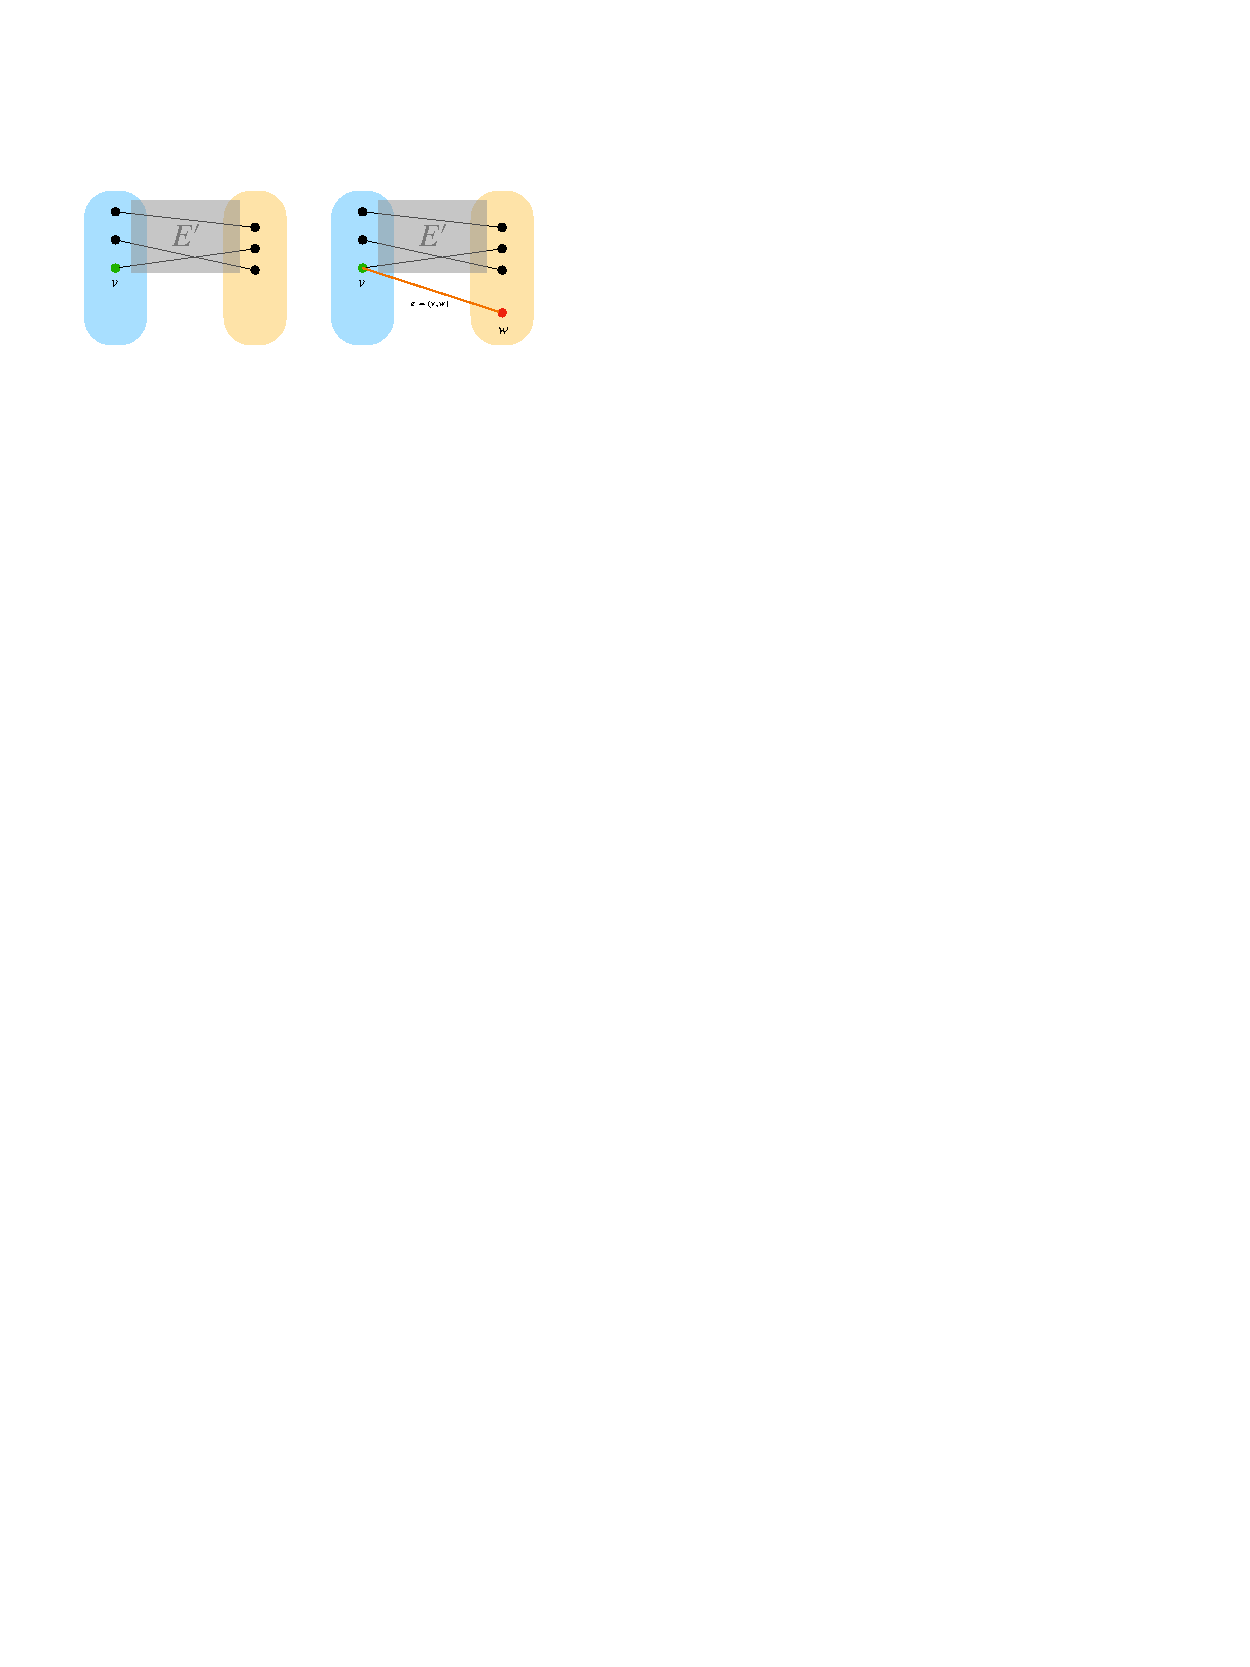
\includegraphics{assets/non-blocking-networks.pdf}}
{\caption{\small The figure above demonstrates the third property of non blocking bipartite graphs $G=(L\cup R, E)$. As $E' \subseteq E$ is a safe state that is not too large, by the non blocking property, we are \emph{guranteed} to connect any vertex $v \in L$ to a vertex $w \in R$ that has no incident edges from $E'$.}
}
\label{fig:test}

\end{figure}

Next, we re-state a lemma by \citep[Proposition 1]{feldman1988wide} which describes the properties bipartite graphs must satisfy to be non-blocking.

\begin{lemma}\label{lemma:condtions-for-non-block}
Fix $a, r, s \in \Naturals$. Let $\Graph = (A \cup B, E)$ be a bipartite graph.
If for every $X \subseteq A$ of size $1 \leq |X| \leq 2a$, there are \emph{at least} $(r + s)|X|$ vertices in $B$ that are adjacent to some vertex in $S$, \emph{then}, $\Graph$ is $(r, as)$-non blocking.
\end{lemma}


\section{Proof Of Main Result}
\label{sec:main-proof}

Let $G=(V,E)$ denote any $\EnDeeLambda$-graph on an odd number of vertices, and,  $\HardInstance$ denote the hard instance on $t=\BigO{\frac{n}{\log n}}$ vertices for polynomial calculus known to exist as per Lemma \ref{lemma:worst-case-instance-PC}.
The hardness proof follows from the following steps, and is illustrated in Figure \ref{fig:proof-outline}.


\begin{figure}
  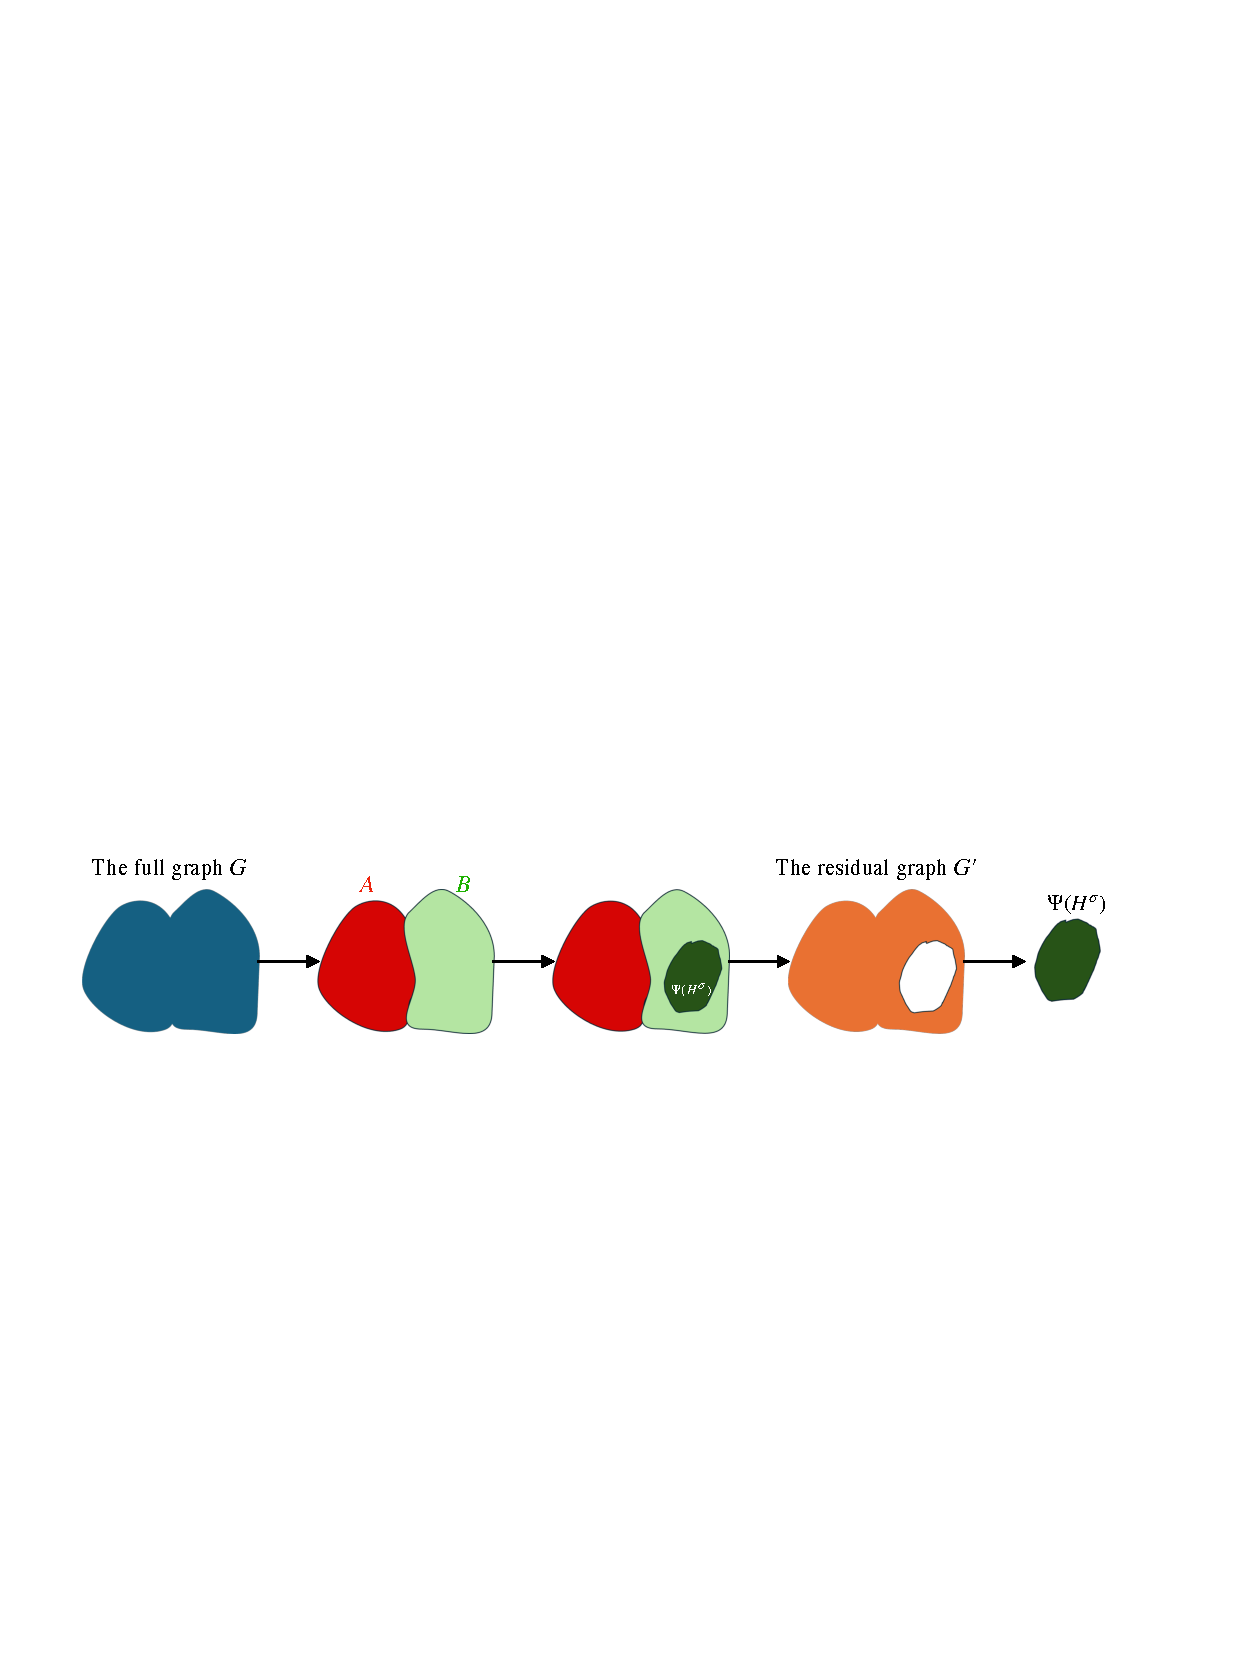
\includegraphics[width=0.8\textwidth]{assets/proof-sketch.pdf}
  \caption{The figure above above outlines the steps of the proof. First we partition the vertices of $G$ into balanced sets $\RedA$ and $\GreenB$. After that, we topologically embed the hard instance $H$ such that every path representing an edge of $e$ in the embedding is of odd size. This ensures that the graph restricted to the embedding is hard to refute. Next we show that the induced subgraph (referred to as the residual graph $\RemGraph = G[V \setminus \Embedding{\Subdivision{H}{\sigma}}]$) has a perfect matching. This  implies that the hardness to refute matchings in $G$ is transferred to the hardness of refuting $H$.} 
	\label{fig:proof-outline}
\end{figure}

\begin{enumerate}
\item{First, we show (via Theorem \ref{thm:partition}) that we can partition the vertices of the graph $\Graph$ into two disjoint sets $\RedA$ and $\GreenB$, as shown in Figure \ref{fig:partition}, of roughly equal size.
    Apart from $\RedA$ and $\GreenB$ being roughly the same size, the partition has the property that for each vertex $v \in V$ has roughly the same number of neighbours in $\RedA$ and $\GreenB$.
    We formalise what ``roughly'' equal means in Section \ref{sec:partition-lemma}.
    Given this partitioning, we will topologically embed $H$ into the subgraph $G_{\GreenB}$ which is described by the edges of $G$ where both endpoints lie in $\GreenB$. 
  }
  
\item{Let $D = d/\lambda \in \Reals$. We find a subdivision  $\Subdivision{H}{\sigma}$ of $H$, where for each $e \in \Edges{H}$, we have $\sigma(e)  \Def 2k+1$ for $k = \BigO{\log_{D} n}$.
    We show (via Theorem \ref{thm:top-embedding}) that $\Subdivision{H}{\sigma}$ is a subgraph of $G_{\GreenB}$ defined above.
    Let $\EmbeddingFunc: \Vertices{\Subdivision{H}{\sigma}} \rightarrow \Vertices{G_{\GreenB}}$ denote the topological embedding of $H$ into $G_{\GreenB}$, and $G_{\EmbeddingFunc}$ embedded subgraph.
    For each edge $(u,v) \in \Edges{H}$, let $\Path{\Embedding{u}}{\Embedding{v}}$ denote the vertex disjoint odd length path in $\Subdivision{H}{\sigma}$ we construct using Theorem \ref{thm:top-embedding}.
    Then it is at least as hard to refute\footnote{Note that this by itself does not guarantee it is hard to refute $\PM{G}$. We need item (3) and this to show hardness in refuting $\PM{G}$.} $\PM{G_{\EmbeddingFunc}}$ as it is to refute $\PM{H}$.
    To see why, map each variable $y_e$ for $e \in \Path{u}{v}$ alternatingly to $x_{uv}$ or $\bar{x}_{uv}$, such that the edges adjacent to $\Embedding{u}$ and $\Embedding{v}$ are set to $x_{uv}$. This is always possible as $\Path{u}{v}$ is off odd length. Observe that this function maps a perfect matching formula  $\PM{G_{\EmbeddingFunc}}$ to $\PM{H}$. Therefore it should be at least as hard to refute $\PM{G_{\EmbeddingFunc}}$ as it is to refute $\PM{H}$.
}
	
	
%	\item Successfully executing the above steps guarantees that $\HardInstance$ exists inside of $\Graph$ as a topological minor. But as described earlier, this does not suffice in showing that $\PerfectMatching{\Graph}$ is also hard to refute. Let $\Embedding{\HardInstance}$ denote the vertices that form the topological embedding of $\HardInstance$ in $\Graph$. We want to show that the induced subgraph $\Graph[\Vertices{\Graph} \setminus \Embedding{\HardInstance}]$ contains a perfect matching. 
	\item Lastly, we show (via Theorem \ref{thm:perfect-matching}) that the induced subgraph of $G$ not participating in the topological embedding above, has a perfect matching $M$. Define map $\rho: \{x_1, \dots, x_{|\Edges{G}|}\} \rightarrow \{x_1, \dots, x_{|\Edges{G}|}, \bar{x}_1, \dots, \bar{x}_{|\Edges{G}|}, 1, 0 \}$ such that 
	
	\[
        \rho(x_e)=
        \Bigger[10]\{\begin{array}{@{}cl}
                1 & \text{ if $e \in M \land e \notin \Edges{G_{\EmbeddingFunc}}$} \\
                0 & \text{ if $e \notin M \land e \notin \Edges{G_{\EmbeddingFunc}}$}\\ 
                x_e & \text{ otherwise} 
        \end{array}
\]

	If it easy to see that $\PM{G} \equiv \PM{G}|_\rho \equiv \PM{H}$. Therefore by Lemma \ref{lemma:affine_restriction} above, we get that $\PM{G} \in \BigOmega{|\Vertices{H}|} = \BigOmega{\frac{n}{\log n}}$. 

  \end{enumerate}

\subsection{Step 1: Balanced Partitions}
\label{sec:partition-lemma}


These lemmas are referenced from \citet[Chapter 1, Chapter 7]{mitzenmacher2017probability}.
A dependency graph for a set of events $E_1, . . . , E_n$ is a graph $G=(V, E)$ such that $V = \{1,.. . , n\}$ and,  for $i= 1,\dots, n$, event $E_i$ is mutually independent
of the events $\{E_j | (i, j) \notin E\}$. The degree of the dependency graph is the maximum degree of any vertex in the graph.


\begin{lemma}[Multiplicative Chernoff lemma]\label{lemma:mult-chernoff}
Suppose $X_1, ..., X_n$ are identical independent random variables taking values in $\{0, 1\}$. Let $X$ denote their sum and let $\mu = n\Mean{}{X_1}$ denote the sum's expected value. Then for any $0 < \delta < 1$

\[ \Prob{|X - \mu| \geq \delta \mu} \leq 2\exp(-\delta^2\mu/3)\]
	
\end{lemma}




\begin{lemma}[Lov\`asz Local Lemma]\label{lemma:lll}Let $\Dist \in \DistSet{\bit^*}$ be a discrete probability distribution over bit strings of finite length.
  Let $E_1,...,E_n$ be a set of events, and assume that the following hold:
\begin{enumerate}
\item The degree of the dependency graph given by $(E_1, \dots, E_n)$ is bounded by $d$.

\item For all $i \in [n]$, $\PProb{E_i}{\Dist} \leq \beta$

\item $\beta \leq \frac{1}{4d}$, then 
  
\end{enumerate}

\[ \PProb{\overset{n}{ \underset{i=1}{\cap}} \hspace{0.1cm}  \overline{E_i}}{\Dist} > 0\]		


\end{lemma}

Next we describe what it means to have a balanced cut of $G$.
A balanced partition or cut of graph $G$ into sets $\RedA$ and $\GreenB$ is one where both sets are roughly equal in size, and have roughly the same number of edges incident on them.

\begin{figure*}
    \centering
    \begin{subfigure}[t]{0.45\textwidth}
        \centering
        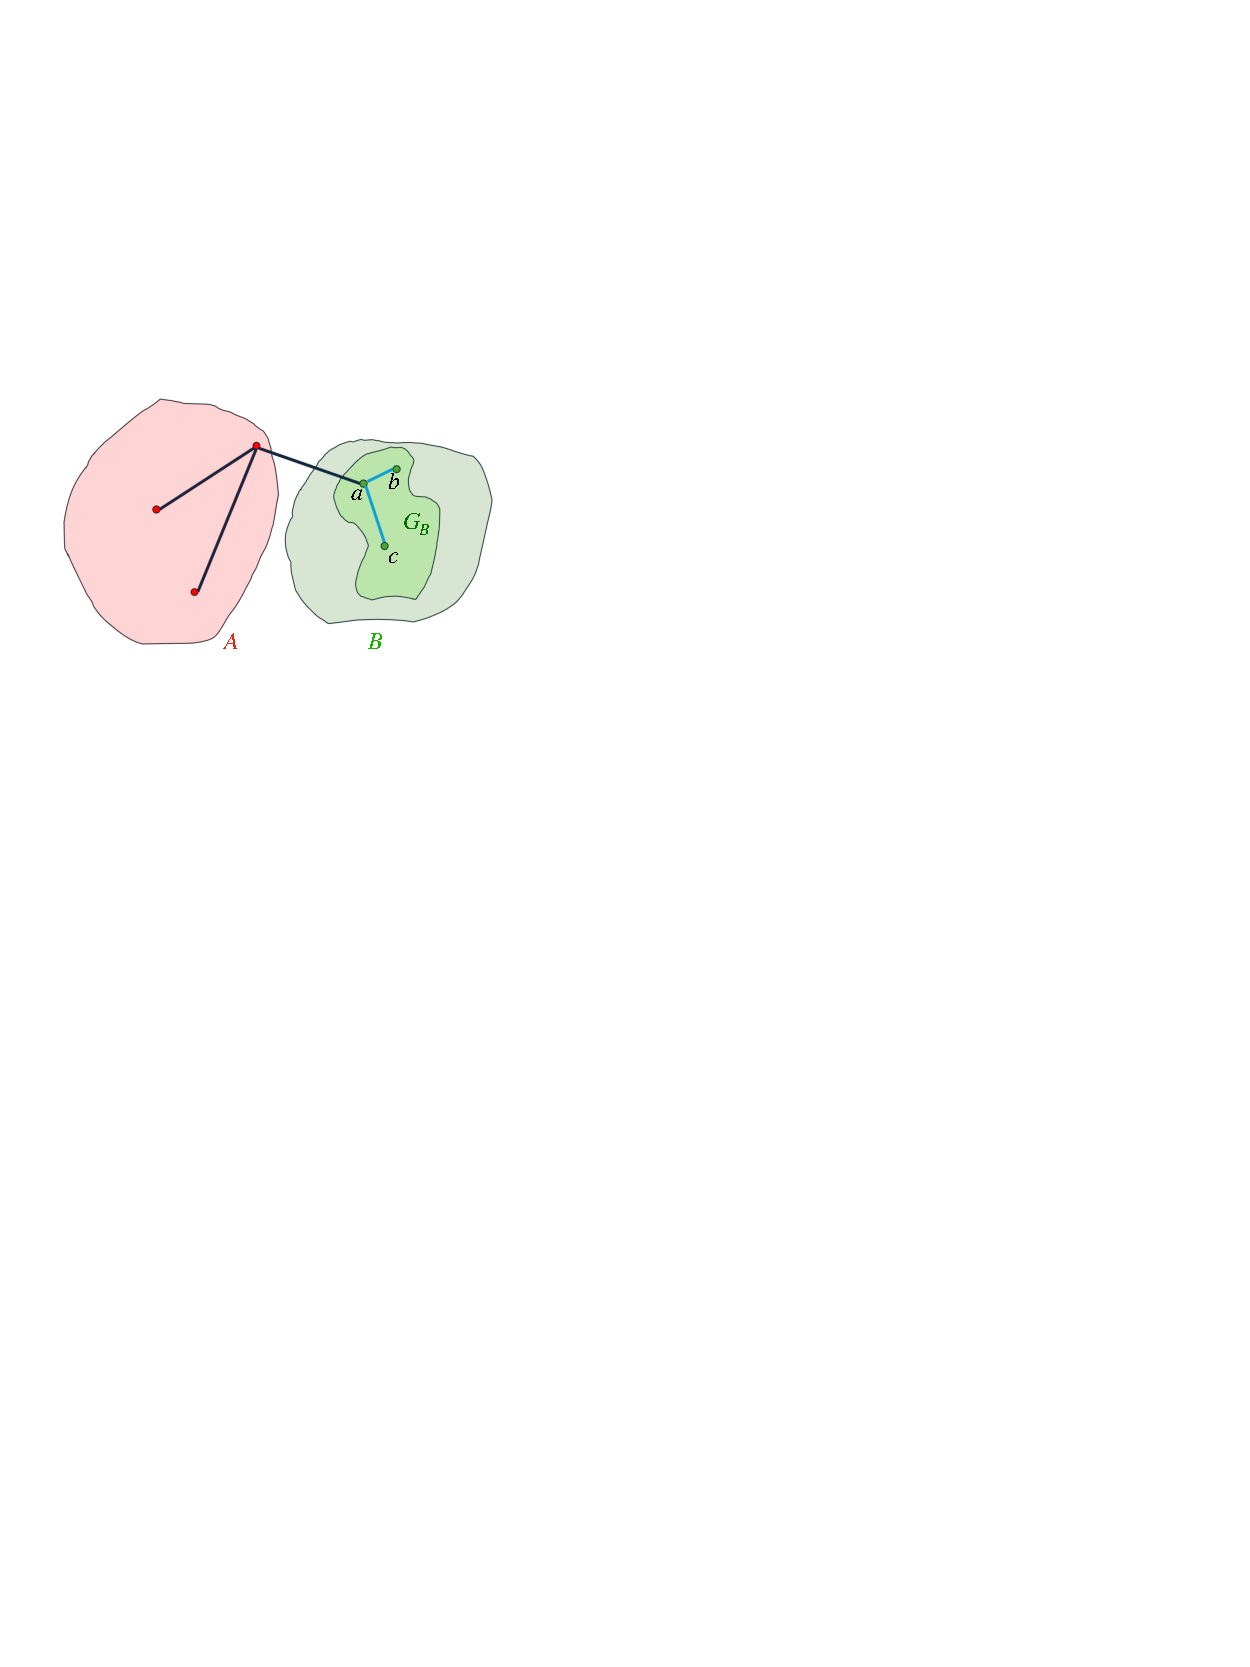
\includegraphics[width=\textwidth]{assets/partition-a.pdf}
        \caption{}
      \label{fig:partition}
    \end{subfigure}%
    \hspace{1mm}
    \hspace{1mm}    
    \begin{subfigure}[t]{0.45\textwidth}
        \centering
        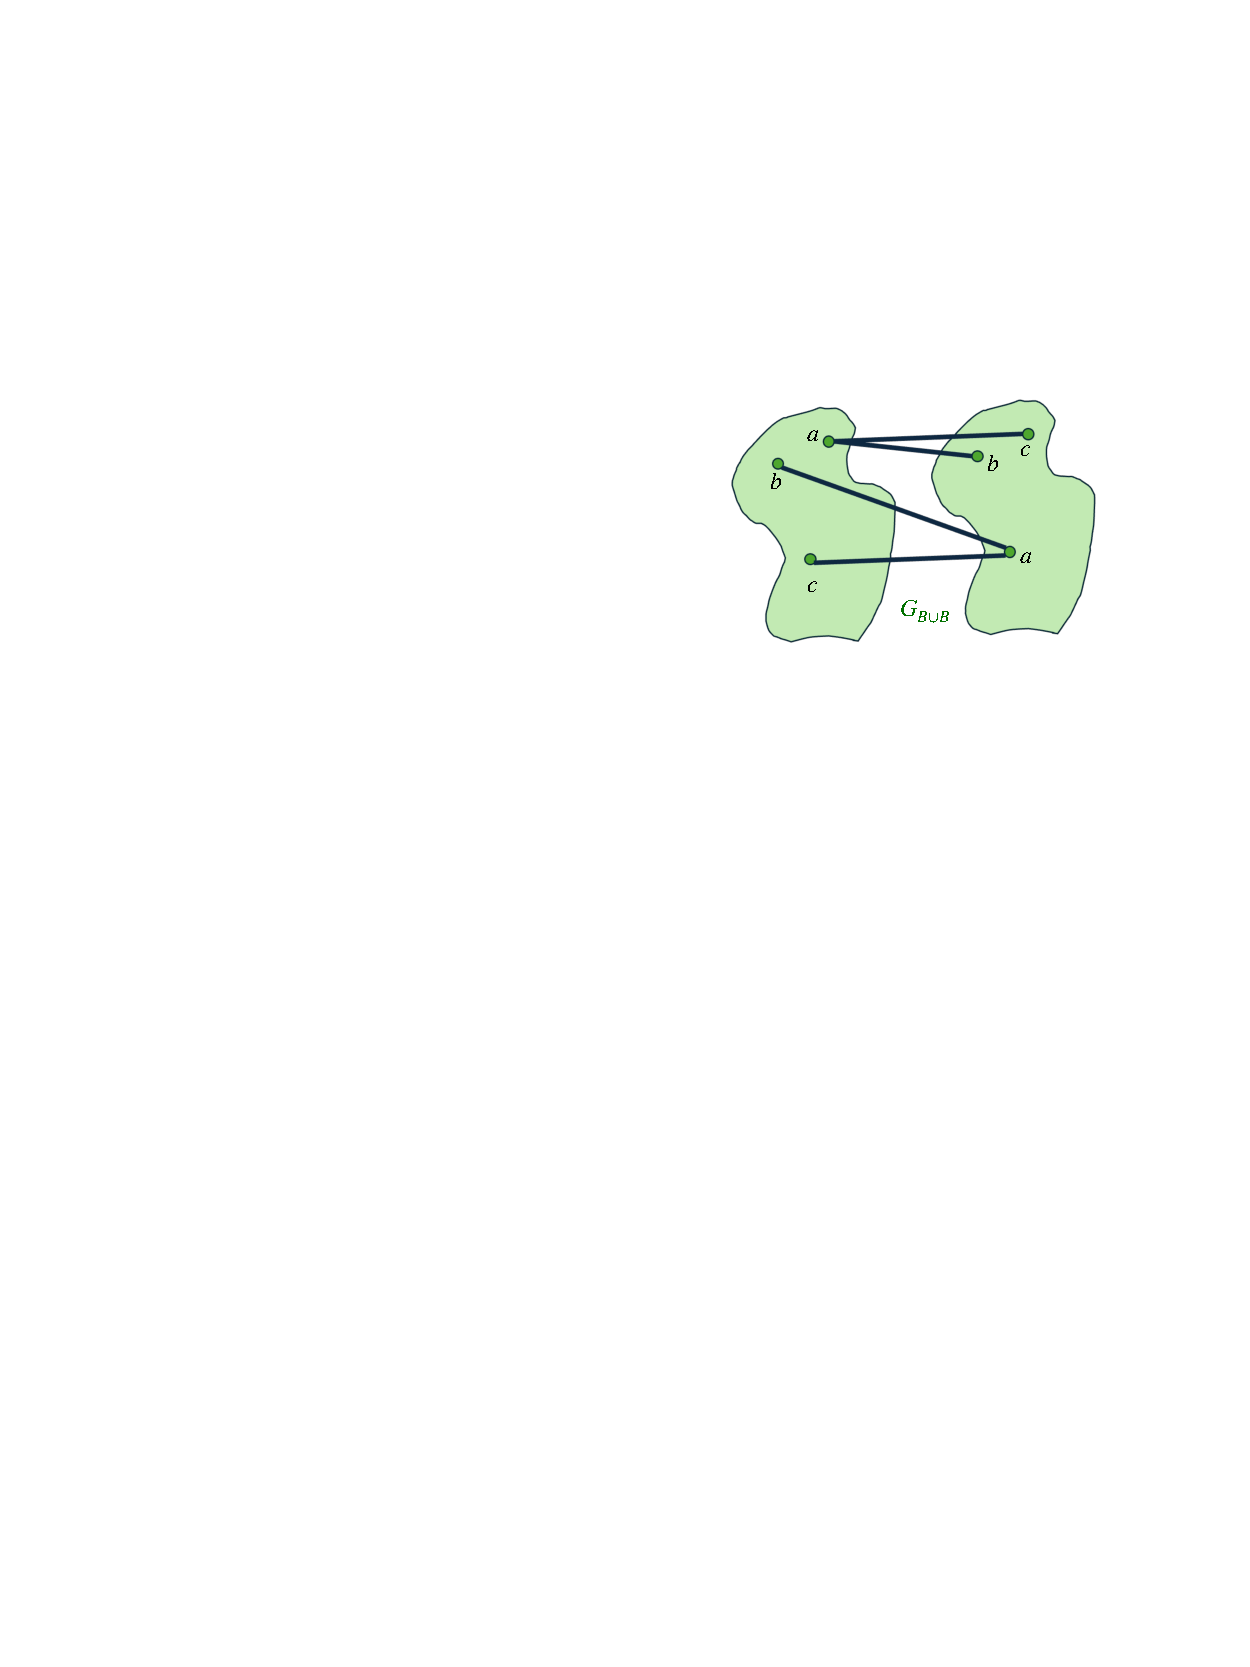
\includegraphics[width=\textwidth]{assets/partition-b.pdf}
        \caption{}
      \label{fig:bipartite}        
    \end{subfigure}
    \caption{\small The figure above describes the partitioning of the vertices of the graph $G$ into two sets $\RedA$ and $\GreenB$, such that for every vertex $v \in \Vertices{G}$ has at least $11d/16$ \red{red} neighbours and at most $13d/16$ \red{red} neigbhours. The subgraph $G_{\GreenB}$ obtained by including vertices in $\GreenB$ and edges that stay inside $\GreenB$. The figure on the right, depicts how the subgraph $G_{\GreenB}$ can be expressed as a bipartite graph $\BipartiteG$.}
    \hspace{1mm}     
\end{figure*}


\begin{definition}[Balanced Cuts]\label{defn:balanced-cuts} Given universal constants $0 \leq c \leq 1$ and $\epsilon > 0$, a $(c, \epsilon)$-degree balanced cut of a graph $G$ is apartition $\RedA \cup \GreenB$ ofthe $n$ vertices of $G$, such that, for every vertex $u \in \Vertices{G}$,  $cd - \epsilon d \leq \Neighbourhood{E}{v} \cap \RedA \leq cd + \epsilon d $    
\end{definition}

If a graph on $n$ vertices is $d$-reguar and has a balanced cut $\RedA$ and $\GreenB$, then $\frac{\Size{\RedA}}{\Size{\GreenB}} = \BigO{1}$. In other words $\Size{\RedA}, \Size{\GreenB} \in \BigO{n}$ i.e $\RedA$ and $\GreenB$ are roughly the same size.

\begin{remark}
  Throughout the rest of this document, for any $(c, \epsilon)$ balanced partition $\RedA \cup \GreenB$ of any graph $G$,  we describe vertices in $\RedA$ as \red{red} nodes, and vertices in $\GreenB$ as \green{green} nodes.
\end{remark}

The proof for the following theorem is a textbook application of the  \nameref{lemma:lll} along with the \nameref{lemma:mult-chernoff}.
The main contribution lies in how we use the balanced cuts to get a perfect matching in the residual graph in Theorem \ref{thm:partition} i.e step 3 of the proof.

\begin{lemma}[Pseudorandom Graphs Have Balanced Cuts]\label{thm:partition}
For every $0 < c < 1$, and $\epsilon > 0$, there exists a constant $d_0 \in \BigOTilde{c/\epsilon^2}$, such that, given a $d$-regular graph $\Graph = (V, E)$ on $n$ vertices, with $d \in [d_0, n-1]$, there exists and a  sets $\red{A}$ and $\green{B}$ is a $(c, \epsilon)$ balanced cut of $G$.
\end{lemma}

\begin{proof}
We prove the existence of such a partition $\RedA \cup \GreenB = V$ using the probabilistic method.
For each $v \in \Vertices{\Graph}$, we toss an independent coin $X_i$ with bias $c$.
If $X_i = 1$, then we include $v$ in $\RedA$, else we put $v$ in $\GreenB$.
Thus, $\vec{X} \Def (X_1, \dots, X_n) \in \bit^n$ is a random variable that describes how we partition $V$ into sets $\RedA$ and $\GreenB$.
For any $v \in V$, let $Y_v \Def |\Neighbourhood{E}{v} \cap \RedA|$ denote the random variable that counts how many \red{red} neighbours of $v$ has.
Define $\delta \Def \frac{\epsilon}{c}$, and for any $v \in V$, let $E_v = \Indicator{|Y_v - d c | \geq \delta c d}$ denote the bad event that $v$ has too many \red{red} neighbours.
Observe that the dependency graph of events $\{ E_v \}_{v \in V}$ has max-degree at most $d^2$.
To see why, for any node $v$, let $u$ and $w$ denote vertices exactly 2 hops\footnote{A node $a$ is $k$ hops away from another node $b$ if the shortest path between $a$ and $b$ has $k$ eges.} and at least 3 hops away from $v$ respectively. The colour of $u$'s neighbours, directly affects how many red neighbours $v$ can have.
However, as the colours for each node is sampled independently, the colour of $w$ or its neighbours do not affect $v$'s neighbours.
Therefore $E_v$ is independent of $E_w$.
There are at most $d^2$ nodes at a distance of at most 2 from any node, giving us the max-degree of the dependency graph.
As $\Graph$ is $d$-regular, $\Mean{\vec{X}}{Y_v} = c d$, then by the \nameref{lemma:mult-chernoff}, for any $v \in V$, we have $\PProb{E_v}{\vec{X}} \leq 2\exp(-\delta^2c d/3) \Def \beta$.
There exists $d_0 \in \BigOTilde{c/\epsilon^2}$, such that for $d > d_0$, for some $d_0$, we have that $2\exp(-\delta^2c d/3) \leq 1/(4d^2)$. Therefore, we have $\beta d^2 \leq 1/4$.
We have all the conditions to invoke the \nameref{lemma:lll} to get $\PProb{\underset{{v\in V}}{\land}E_v = 0}{\vec{X}} > 0$.
\end{proof}

\subsection{Step 2: The Topological Embedding}

\begin{remark}
  \label{remark:edge-dist}
For this section, and the next, we invoke Lemma \ref{thm:partition} with parameters.  $c=3/4$ and $\epsilon=1/16$.
Reviewing the properties of a balanced sets with $c=3/4$ and $\epsilon=1/16$, we have that every vertex $u$ in any $\EnDeeLambda$ graph  $G=(V,E)$,

\begin{align*}
\text{ Number of \red{red} neighbours:} \quad &\frac{11}{16}d  \leq   \Size{\Neighbourhood{E}{u} \cap \RedA} \leq \frac{13}{16}d \\
\text{ Number of \green{green} neighbours:} \quad & \frac{3}{16}d  \leq   \Size{\Neighbourhood{E}{u} \cap \GreenB} \leq \frac{5}{16}d \\
\end{align*}
  
\end{remark}

Given $\EnDeeLambda$ graph $G=(V,E)$, let $\RedA$ and $
\GreenB$ be the partition guaranteed by the \ref{thm:partition}.
Define $E_{\GreenB} \Def \{ (\green{u},\green{v}) \in E : \green{u} \in \GreenB \land \green{v} \in \GreenB\}$. 
That is $E_{\green{B}}$ is the set of edges whose endpoints are fully contained in B (they have \green{green} endpoints), and let $G_{\green{B}}$ be the subgraph defined by the edges $E_{\GreenB}$. 
Define $ \na \Def |G_{\GreenB}|$, which by the balancedness of the partition is some constant fraction of $\Size{V}$.
Now define a bipartite graph $\BipartiteG = \left(\Vertices{\GreenB} \cup \Vertices{\GreenB}, E_{\GreenB} \right)$ (see Figure \ref{fig:bipartite}).
That is the left and right vertices of $\BipartiteG$ are copies of $G_{\GreenB}$ and for every edge $(u,v) \in E_{\GreenB}$, there is a corresponding copy $(u,v) \in \Edges{\BipartiteG}$.

\begin{remark}
  
To avoid notation clutter, we will refer to the left and right vertex sets of $\BipartiteG$ with $X$ and $Y$ respectively.
Also by definition, every vertex in $X$ and $Y$ \emph{must} be \green{green}.  
\end{remark}

\begin{lemma}\label{lemma:bipartitie-is-non-blocking}Let $G$ be the $\EnDeeLambda$ graph given to us and let $\BipartiteG$ be the bipartite graph constructed using the balanced partition theorem. 
There exists small universal constants $\epsilonL, \epsilonA  \in (0,1)$ independent of $d$ and $n$, such that if $\lambda < \epsilonL d$, then $\BipartiteG$ is $(\frac{d}{\lambda}, \epsilonA n)$ non-blocking.
\end{lemma}

\begin{proof}
Let $\BipartiteG \Def (X \cup Y, E_{\GreenB})$. 
Let $\lambda \Def \ExpansionFactor{G} \leq d/c_2$ where $c_2 > 0$ is a constant to be defined shortly.
Set $a = \frac{n\lambda}{2c_1 d}$ for a constant $c_1 > 0$ to be defined next.
Set $c_1, c_2$ such that $\left(\frac{1}{c_1/2}  + \sqrt{\frac{1}{c_2/2}}\right) < \frac{3}{16}$.
Pick any $S \subseteq X$ with $|S| \leq 2a = \frac{n\lambda}{c_1 d}$.
\highlight{Assume towards a contradiction} that $\BipartiteG$ is \textbf{not} non-blocking.
  Then by Lemma \ref{lemma:condtions-for-non-block} there exists a set $T \subseteq Y$, adjacent to some vertex in $S$ such that $|T| < |S|(\frac{d}{\lambda}+\frac{d}{\lambda})$. 
By the balanced cut property we know that, every \green{green} node is connected to at least $\frac{3}{16}d$ \green{green} nodes (and $E_{\GreenB}$ consists of all edges with two \green{green} endpoints) i.e.

\begin{equation}\label{eq:balanced}
  \CutEdges{S}{T}{E_{\GreenB}} \geq \frac{3}{16}|S|d
\end{equation}

However, $S$ and $T$ are also subsets of $\Vertices{G}$ and $G$ is a $\EnDeeLambda$ graph.
From the \nameref{lemma:expanders-mixing-lemma}, we have

\begin{align}
	\CutEdges{S}{T}{E_{\GreenB}} &\leq \frac{d}{n}|S||T| + \lambda\sqrt{|S||T|} \\
	&< 2\frac{2d^2}{n\lambda}|S|^2 + |S|\sqrt{2\lambda d} \label{eq:assumption}\\
	&\leq |S|\left(\frac{2d^2}{\lambda n} \frac{n\lambda}{c_1 d} + \sqrt{d\cdot \frac{d}{c_2/2}}\right) \label{eq:assumption-lambda}\\
	&= |S|d\left(\frac{1}{c_1/2}  + \sqrt{\frac{1}{c_2/2}}\right) \\
	&< |S|d\frac{3}{16} \label{eq:constants}
\end{align}

\eqref{eq:assumption} comes from our \highlight{assumption}.
\eqref{eq:assumption-lambda} comes from our assumption that $\lambda \leq d/c_2$ and $|S| \leq \frac{n\lambda}{c_1 d}$.
\eqref{eq:constants} contradicts the balanced sets property in Equation \eqref{eq:balanced}, so our \highlight{assumption} must have been wrong.
Finally we get our theorem statement by setting $\epsilonL = 1/c_2$ and $\epsilonA = 1/c_1$.

\end{proof}

With the non-blocking nature of $\BipartiteG$ established, the next step is to embed hard instance $H$ as topological minor of $\GreenB$ as described in the overview.
Note for every edge in $E_{\GreenB}$, by our construction, we will have a corresponding edge in the bipartite graph $\BipartiteG$.


\begin{definition}[Sub-divisions]\label{def:subdivisions}
Given a graph $H$ and a function $\sigma: \Edges{H} \rightarrow \Naturals$, the $\sigma$-subdivision $H$, denoted by $\Subdivision{H}{\sigma}$, is the graph obtained by replacing each edge in $\Edges{H}$ with a path of length $\sigma(e)$ joining the end points of $e$ (such that all these paths are mutually vertex disjoint, except at the end points).	
\end{definition}

\begin{definition}[Topological Minor]\label{def:topological-minor}
A graph $H$ is a topological minor of a graph $G$ if there exists a subdivision $\Subdivision{H}{\sigma}$ that is isomorphic to \emph{any} subgraph of $G$.	
\end{definition}

\begin{theorem}[Topological Embedding Theorem]\label{thm:top-embedding}
Let $G$ be a $\EnDeeLambda$ graph, and $\BipartiteG$ be the construction defined from the balanced partition theorem, where $|\GreenB| = \na$.
Let $H$ be the worst case hard instance on $t = \lceil\epsilonA \frac{\na}{\log \na}\rceil = \BigO{\frac{n}{\log n}}$ vertices known to exist in Lemma \ref{lemma:worst-case-instance-PC}, where $0 < \epsilonL < \epsilonA <1$ are the constants from  Lemma \ref{lemma:bipartitie-is-non-blocking}.	
If $\lambda \leq \epsilonL d$, then $G$ contains a subdivision of $H$, denoted by $\Subdivision{H}{\sigma}$ as a subgraph.

\end{theorem}



\begin{proof}
Define $D = \frac{d}{\lambda}$ and $k \Def \lceil\log_D\na\rceil$.
Let $\{ h_1, \dots, h_t\}$ denote the vertices of $H$.
Define $\sigma(e) \Def \PathSize \Def 2k+1$ for all $e \in \Edges{H}$.
Let $\EmbeddingFunc: \Vertices{\Subdivision{H}{\sigma}} \rightarrow \Vertices{G_{\GreenB}}$ be the bijective mapping between the vertices of $\Subdivision{H}{\sigma}$, and the vertices of $G_{\GreenB}$, that defines our topological embedding.
Our first task is to find a unique $\Embedding{h} \in \Vertices{G_{\GreenB}}$ for each $h \in \Vertices{H}$.
Let $\{a_1, \dots, a_{t}\}$ be arbitrary set of $t$ vertices in $\Vertices{G_{\GreenB}}$.
Let $X=\Vertices{G_{\GreenB}}$ and $Y=\Vertices{G_{\GreenB}}$ denote the left and right sides of the bipartite graph $\BipartiteG$ described above.
We repeat the following process to obtain $\{ \Embedding{h_1}, \dots, \Embedding{h_t}\}$: 

\begin{figure*}[t!]
    \centering
    \begin{subfigure}[t]{0.95\textwidth}
        \centering
        \includegraphics{assets/embeddingA.pdf}
        \caption{The \textcolor{purple}{purple} edges represent the edges in $\cup_{i=1}^j (M_j \cup M_j')$, which we have already included in the $\GlobalEdgeSet$.
        For any $v$ in $S_j \subseteq X$ (\textcolor{cadmiumgreen}{green vertex}) we ask for $D$ neighbours in $S_{j+1} \subseteq Y$ (shown with \textcolor{cadmiumgreen}{green} and \textcolor{carminepink}{pink} lines). 
        Of these $D$ edges, by the non-blocking property, we know that there will be at least one edge (in this case there are 3 such edges shown in \textcolor{carminepink}{pink}) such that the endpoints in $Y$ are not connected to any of the \textcolor{purple}{purple} edges in $\GlobalEdgeSet$ . 
        The \textcolor{cadmiumgreen}{green} dotted edges are unsafe, so we cannot use them. We will add the safe \textcolor{carminepink}{pink} edges to $M_j$.}
        \label{subfig:embeddingA}
    \end{subfigure}%
    \hspace{1mm}
%    \vrule width 1pt % vertical line
    \hspace{1mm}
    \begin{subfigure}[t]{0.95\textwidth}
        \centering
        \includegraphics[]{assets/embeddingB.pdf}
        \caption{We restrict the size of $M_j$ to be $\min\{t, |S_{j-1}|D\}$ edges. As $k = \log_{D}[\na]$, eventually, for some $j \leq k$, we get $t \leq |S_{j-1}|D$.
        In the above example $M_{j-1}$ has size $D|S_{j-2}|$ but $M_j$ has size $t$. 
        From then on for all $j \leq i \leq k$, $|M_i|= t$.
        Furthermore, for $j \leq i \leq k$,  each vertex in $S_i$ will be connected to exactly one vertex in $S_{i+1}$ via a safe edge.
        }
        \label{subfig:embeddingB}        
    \end{subfigure}
\end{figure*}




\begin{itemize}
\item Define $E' = \emptyset$ to begin with, and as $\BipartiteG$ is a $(D, \epsilonA n)$-non blocking bipartite graph (by Lemma \ref{lemma:bipartitie-is-non-blocking}), $E'$ is a \emph{safe} state.
  
\item For $a_1 \in X$, we ask for $D$ neighbours in $Y$. By the non-blocking property, we can find a \emph{safe neighbour} $\tilde{h}_1 \in Y$ such that there is no edge in $E'$ is incident on $\tilde{h}_1$. We set $\Embedding{h_1} \Def \tilde{h}_1$ and update $E' = E'  \cup \{(a_1, \tilde{h}_1)\}$.
  
\item We repeat this process for all $a \in \{a_2, \dots, a_t\}$. For the $j$'th step, As $|E'| = j \leq t < \epsilonA\na$, for each $a_j$ we can always find a \emph{safe neighbour} $\Embedding{h_j} \Def \tilde{h}_j$ in $Y$ such that there is an edge from $a_j$ to $\tilde{h}_j$, and there is no other edge in $E'$ so far, that is incident on each $\tilde{h}_j$.
  
\end{itemize}

Once this phase is complete, we have mapped every vertex of $H$ to a vertex in $G_{\GreenB}$.
That is we have defined $\Embedding{h_i}$ for all $i \in [t]$.
The next step to show that for each $(u,v) \in \Edges{H}$, there is a vertex disjoint path of odd length $\PathSize = 2k+1$ between $\Embedding{u}$ and $\Embedding{v}$ in $G_{\GreenB}$.
Let $(e_1, \dots, e_m)$ be an arbitrary ordering of edges in $\Edges{H}$.
We prove the result by induction on $m$.

\paragraph{Base case} 

Let $e_1 = (u_1,v_1)$. Define sets $S_0 = \{\Embedding{u_1}\}$ and $S'_0 = \{ \Embedding{v_1}\}$, and set $M_0 = \emptyset$ and $M_0' = \emptyset$.
Define a global edge set and set it to $\GlobalEdgeSet \Def \emptyset$.
We will define edge sets $\{ M_j\}_{j \in [k]}$ and $ \{ M'_j\}_{j \in [k]}$, and vertex sets $\{ S_j\}_{j \in [k]}$ and $\{ S'_j\}_{j \in [k]}$ inductively as follows:

For each $1 \leq j \leq k$, we construct $S_{j}$ with the following process:

\begin{itemize}
\item {For each $x \in S_{j-1}$, find the corresponding copy $x \in X$. Ask for $D$ neighbours of $x$ in $Y$ via edges in $E_{\GreenB}$.
    With respect to $\GlobalEdgeSet \cup \Big(\cup_{i=1}^{j} (M_i \cup M'_i)\Big)$, add exactly one \emph{safe} neigbour of $x$, denoted here with $y$, to $S_{j}$, and add the edge $(x,y)$ to $M_j$. Refer to Figure \ref{subfig:embeddingA} for a visual depiction of this process.
    We discuss below why such a safe edge always exists.}
  
\item{Now there might be other safe neigbours for $x \in S_j$ apart from the one we just added. Add these neighbours to $S_j$, and the edges to $M_j$ as long the size of $M_j \leq \min\{t, |S_{z-1}|D\}$.
    Thus, the two extreme cases are the every $x \in S_{j-1}$ gets $D$ neighbours in $S_j$, or every $x \in S_{j}$ gets \emph{exactly} one neighour in $S_j$.
For any index $i \leq k$, once a set $|S_i|=t$, for all remaining indices $j > i$, $S_j$'s are of size $t$ as well, with exactly one edge incident on each $a \in S_j$ from $S_{j-1}$. Figure \ref{subfig:embeddingB} illustrates this idea.
  }

\item{\textbf{Why is there always a safe neighbour}: Let $M = \GlobalEdgeSet \cup \Big(\cup_{i=1}^{j} (M_i \cup M'_i)\Big)$.
The reason we can always construct the sets described above sets is that $|M| \leq 2tk < \epsilonA n$, and as $\BipartiteG$ is $(D, \epsilonA n)$ non-blocking, for any vertex $x \in S_j \subseteq X$, with at most $D$ neighbours in $S_{j+1} \subseteq Y$, we can always find \emph{at least} one $y \in S_{j+1}$, such that $(x,y) \in E_{\GreenB}$ and no edge in $\cup_{i=1}^{j-1} (M_i \cup M'_i)$ is incident on $y$.}  


\end{itemize}



Now as $k = \log_D[n]$, we have that, $|S_k| = |S_k'|= t$.
By the expander mixing lemma \ref{lemma:expanders-mixing-lemma},

\begin{align}
\CutEdges{S_k}{S_k'}{E_{\GreenB}}
 &\geq \frac{d t^2}{n} - \lambda t \\
	&> 0 \label{eq:greater}
\end{align}

Equation \eqref{eq:greater} comes from the assumption $\lambda \leq \epsilonL d$ (from Lemma \ref{lemma:bipartitie-is-non-blocking}).
This implies there exists at least one edge $e^\star=(x^\star,y^\star) \in \CutEdgesSet{S_k}{S_k'}{E_{\GreenB}}$.
By how we constructed $M_k$, we know that $x^\star$ was the safe neighbour of some node $a \in S_{k-1}$.
Let $m_k \Def (a,x^\star) \in M_k$ be the connecting edge.
Similarly, there is some edge $m_{k-1} \in M_{k-1}$ that connects some vertex in $S_{k-2}$ to $a$ with a safe edge.
We repeat this process all the way, till we get $k+1$ edges, $m_1 m_2 \dots, m_k, e^\star$.
We repeat the same process for the other end point of $y \in S_k'$, to get edges $e^\star, m'_1, \dots, m'_k$.
We add these edges to a global edge set $\GlobalEdgeSet$.
Thus, we have found an odd length path $m_1\dots m_k e^\star m_1'\dots m_k'$ of length $2k+1$, connecting $\Embedding{u}$ to $\Embedding{v}$.
 Figure \ref{fig:baseB} illustrates everything discussed so far pictorially.

\begin{figure}
	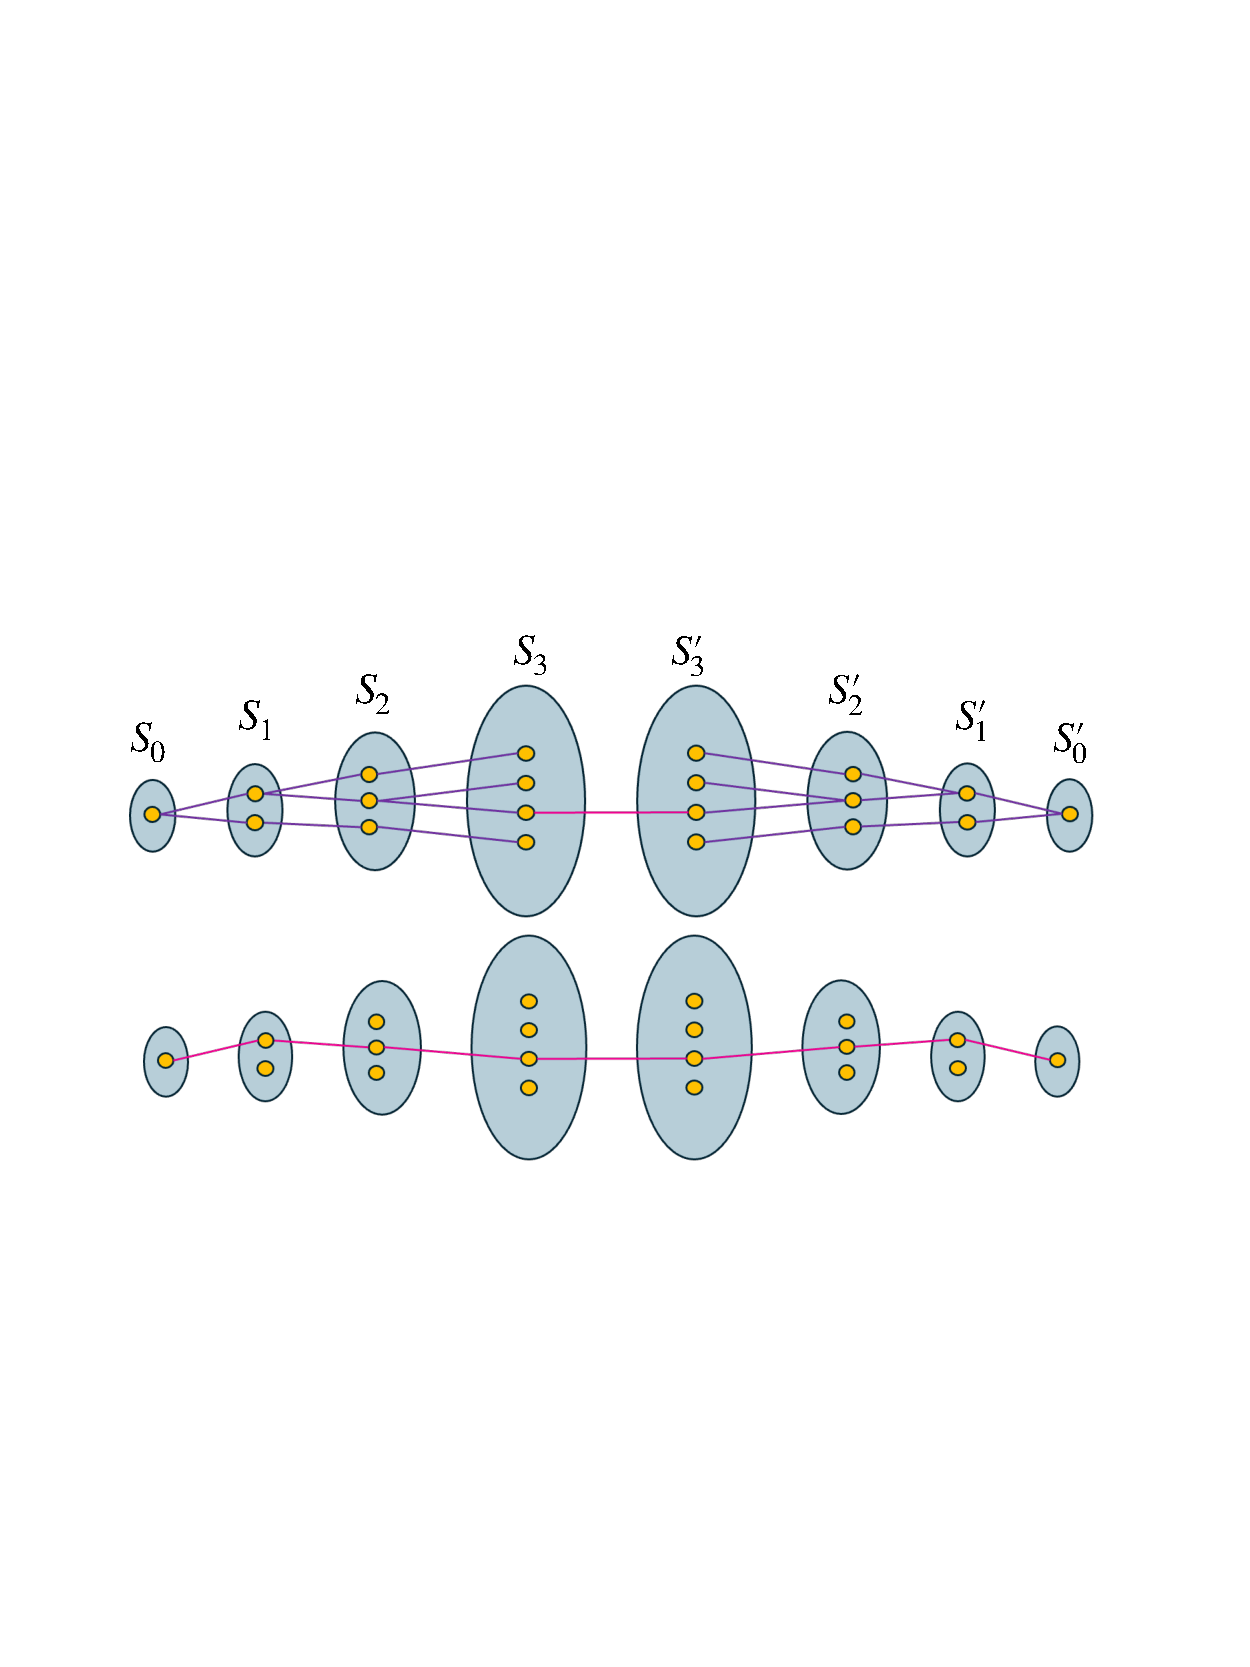
\includegraphics[width=0.9\textwidth
	]{assets/BaseA.pdf}
	\caption{In this toy example, $k=3$. The figure on top describes the forward phase of finding sets $\{M_i\}_{i\in [k]}$ and $\{M_i'\}_{i\in [k]}$. The figure below describes the process of backtracking from the edge $e$ that is promised to exist between $S_k$ and $S_k'$.
    All the edges in pink are added to the global set $\GlobalEdgeSet$.}
	\label{fig:baseB}
\end{figure}



\paragraph{Induction Step}
	
Assume that we have found paths for $e_1 = (u_1, v_1), \dots, e_j=(u_j, v_j)$ for $j < m$.
Let $P_1, \dots, P_j$ denote these paths (depicted with \textcolor{carminepink}{pink} edges in Figure \ref{fig:induction}) .
Let $\GlobalEdgeSet$ denote the set of all edges in these paths.
Let $e_{j+1} = (u_{j+1},v_{j+1}) \in \Edges{H}$.
So far by induction we have $S_0 = \{u_1, \dots, u_j\}$ and $S_0' = \{v_1, \dots, v_j\}$.
Note that $\GlobalEdgeSet \leq tk < \epsilonA n$.
The process for finding a path between $u_{j+1}$ and $v_{j+1}$ reduces the base case.
We add $u_{j+1}$ to $S_0$ and $v_{j+1}$ to $S_0'$.
Now we to add new nodes to $S_{1}$ and $S_{1}'$, we ask for $D$ neighbours of $u_{j+1}$ and $v_{j+1}$.
Then we add at least one safe neighbour of each to $S_1$ and $S_1'$ respectively. As $M = \GlobalEdgeSet \cup \Big(\cup_{i=1}^{j} (M_i \cup M'_i)\Big)$, and $|M| < \epsilonA\na$ as well, we are guaranteed safe neighbours exist for each node (depicted with \textcolor{purple}{purple} edges in Figure \ref{fig:induction})).
This concludes the proof.

\begin{figure}
	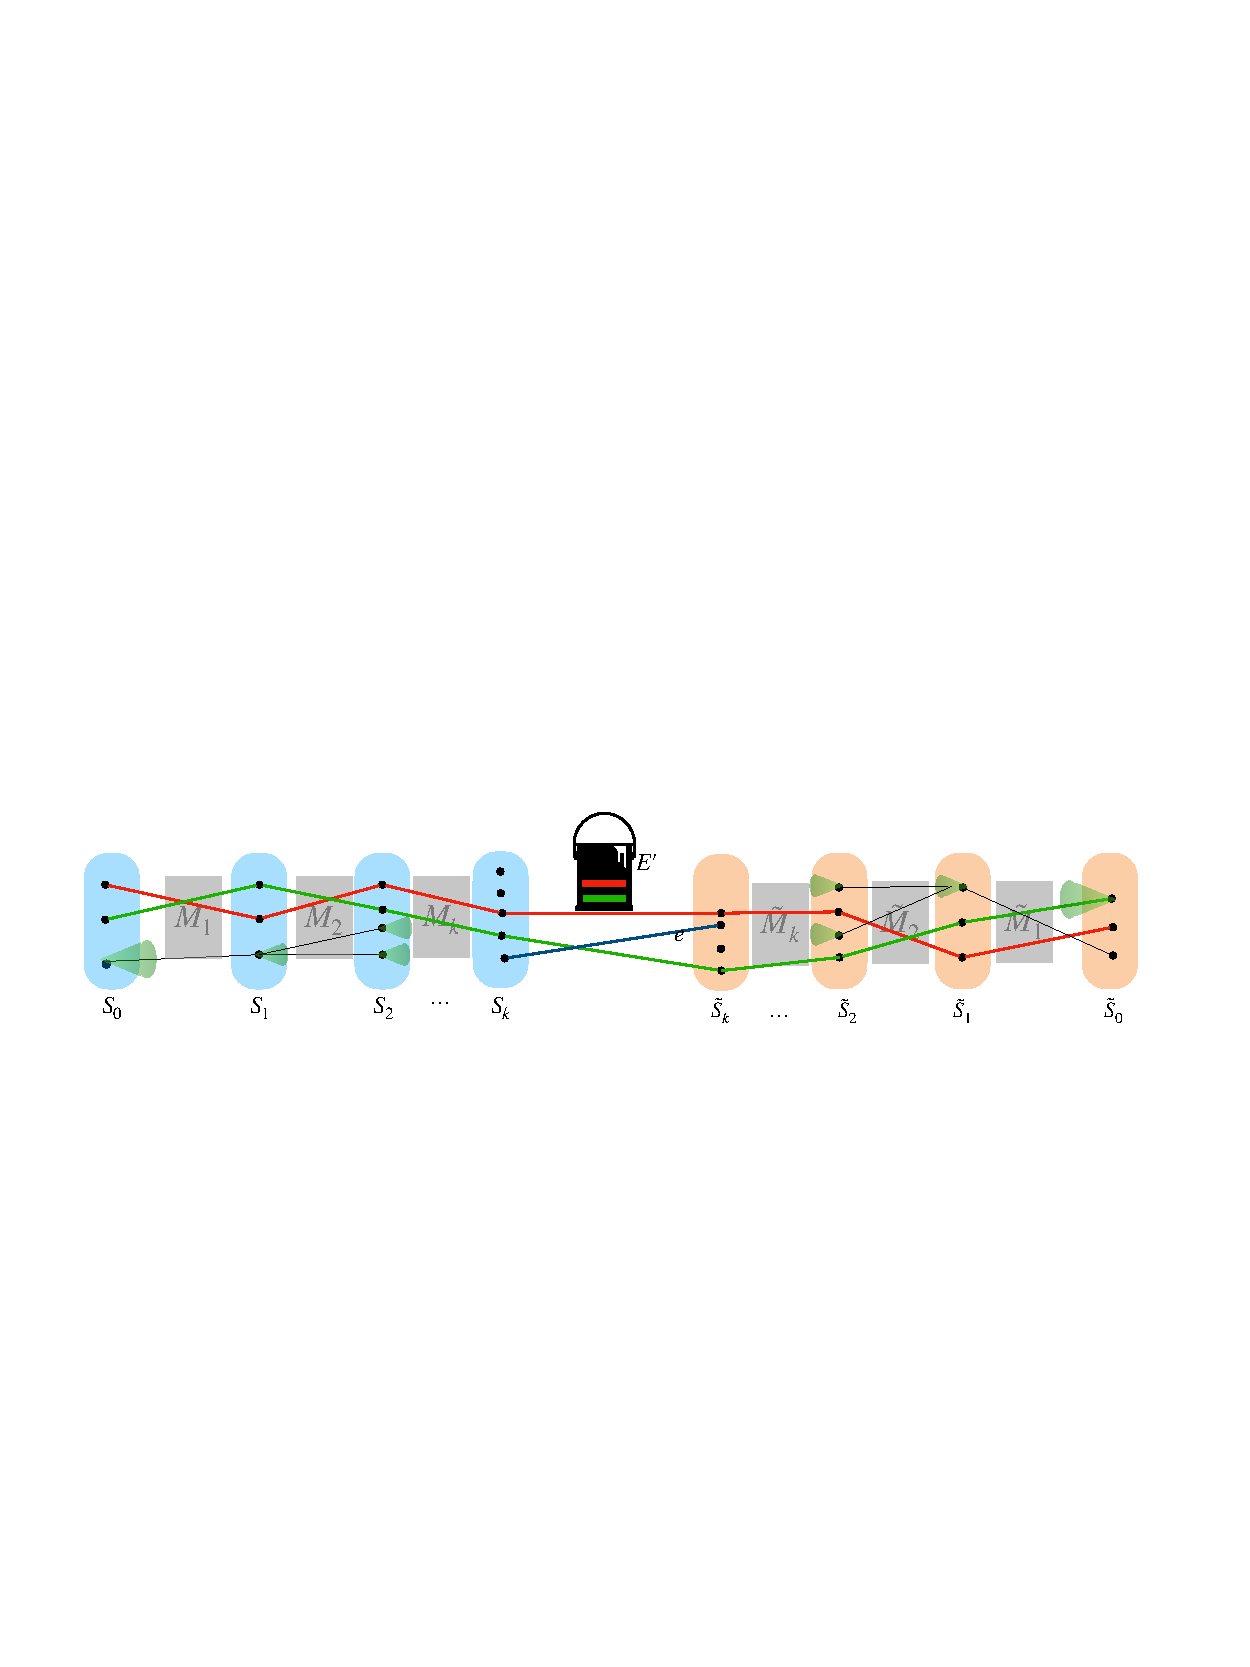
\includegraphics[width=0.9\textwidth
	]{assets/InductionStep.pdf}
	\caption{The figure above describes the induction step. The nodes in green are already in the embedding and represent paths $P_1, \dots, P_j$ for edges $(u_1, v_1) \dots, (u_j, v_j)$.
	The nodes in yellow represent candidates for the path for edge $u_{j+1}, v_{j+1}$. 
	The candidate nodes are constructed identical to the procedure described in the base step of the induction step, where we use the non-blocking property of $\BipartiteG$ to extend with safe neighbours.
    Once we find a blue edge between $S_k$ and $S_k'$, we backtrack like we did in the base case to find the path $\Path{\Embedding{u_{j+1}}}{\Embedding{v_{j+1}}}$.
	}
	\label{fig:induction}
\end{figure}

	
\end{proof}

\subsection{Step 3: Finding A Perfect Matching In The Remainder Of The Graph}

Before describing the full proof, we need some definitions from graph theory.
Proofs for Lemma \ref{lemma:edge-connectivity-pseudorandom} and Lemma \ref{lemma:d-connected-sets-have-no-bad-sets} can be found textbooks \citep{krivelevich2006pseudo}, but we re-derive them as it aids in the understanding of our proof for Theorem \ref{thm:perfect-matching}.

\begin{definition}[Edge Connectivity]\label{def:edge-connectivity}
The edge connectivity of a graph $G$, denoted with $\EdgeConnectivity{G}$ is the minimum number of edges we must delete from the graph to make it disconnected i.e $\EdgeConnectivity{G} = \min_{S \subseteq \Vertices{G}} \CutEdges{S}{\Complement{S}}{\Edges{G}}$
\end{definition}

\begin{lemma}[Edge Connectivity In Pseudorandom Graphs]\label{lemma:edge-connectivity-pseudorandom}
Every $\EnDeeLambda$ graph $G$ with $d - \lambda \geq 2$ has edge connectivity $\EdgeConnectivity{G} = d$.
\end{lemma}
\begin{proof}
  We want to show that for all $S \subseteq \Vertices{G}$ of size $1 \leq \Size{S} \leq \frac{n}{2}$, we have $\CutEdges{S}{\Complement{S}}{\Edges{G}} \geq d$.
  When $1\leq \Size{S} \leq d$, as $G$ is $d$ regular, every vertex in $S$ must have at least $d- \Size{S} + 1$ edges poking out poking out $S$.
  Thus, the total edges out of $S$ is $\Size{S}(d- \Size{S} + 1)$ which has minimal value $d$.
  If $d \leq \Size{S} \leq \frac{n}{2}$, use the tight version of the expander mixing lemma, and combined with the  fact that $d- \lambda > 2$ and $(n-\Size{S})$ is smallest when $\Size{S} = n/2$ to get the bound

  \begin{align*}
    \CutEdges{S}{\Complement{S}}{\Edges{G}} &\geq \frac{d\Size{S}(n-\Size{S})}{n} - \lambda\sqrt{\Size{S}(n-\Size{S}) (1 - \frac{\Size{S}}{n}) (1 - \frac{n-\Size{S}}{n})   }\\
                                            &=  (d-\lambda)(\Size{S}\frac{(n-\Size{S})}{2}) \\
                                              &\geq d
    \end{align*}
  
\end{proof}

\begin{lemma}\label{lemma:d-connected-sets-have-no-bad-sets}
  If $G$ has edge connectivity $\EdgeConnectivity{G} = d$, and $G$ is $d$-regular, then $\forall S \in \Vertices{G}$, $\OddComponents{G \setminus S} \leq |S|$.
\end{lemma}
\begin{proof}
  As $G$ is $d$ regular, any set $S$ has at most $d\Size{S}$ edges incident on it.
  By lemma \ref{lemma:edge-connectivity-pseudorandom}, as $\EdgeConnectivity{G} = d$, every component that connects to $S$ must have at least $d$ edges.
  Therefore the maximum number of components we can have is $\Size{S}$.
\end{proof}

\begin{lemma}[Tutte Criterion]\label{lemma:tutte-criterion}
Let $\OddComponents{G}$ denote the number of odd sized connected components in a graph $G=(V,E)$ with \emph{even} number of vertices.
$G$ admits a perfect matching \emph{if and only if} for every $S \subseteq V$, $\OddComponents{G[V \setminus S]} \leq |S|$.
\end{lemma}
\begin{figure*}
    \centering
    \begin{subfigure}[t]{0.3\textwidth}
        \centering
        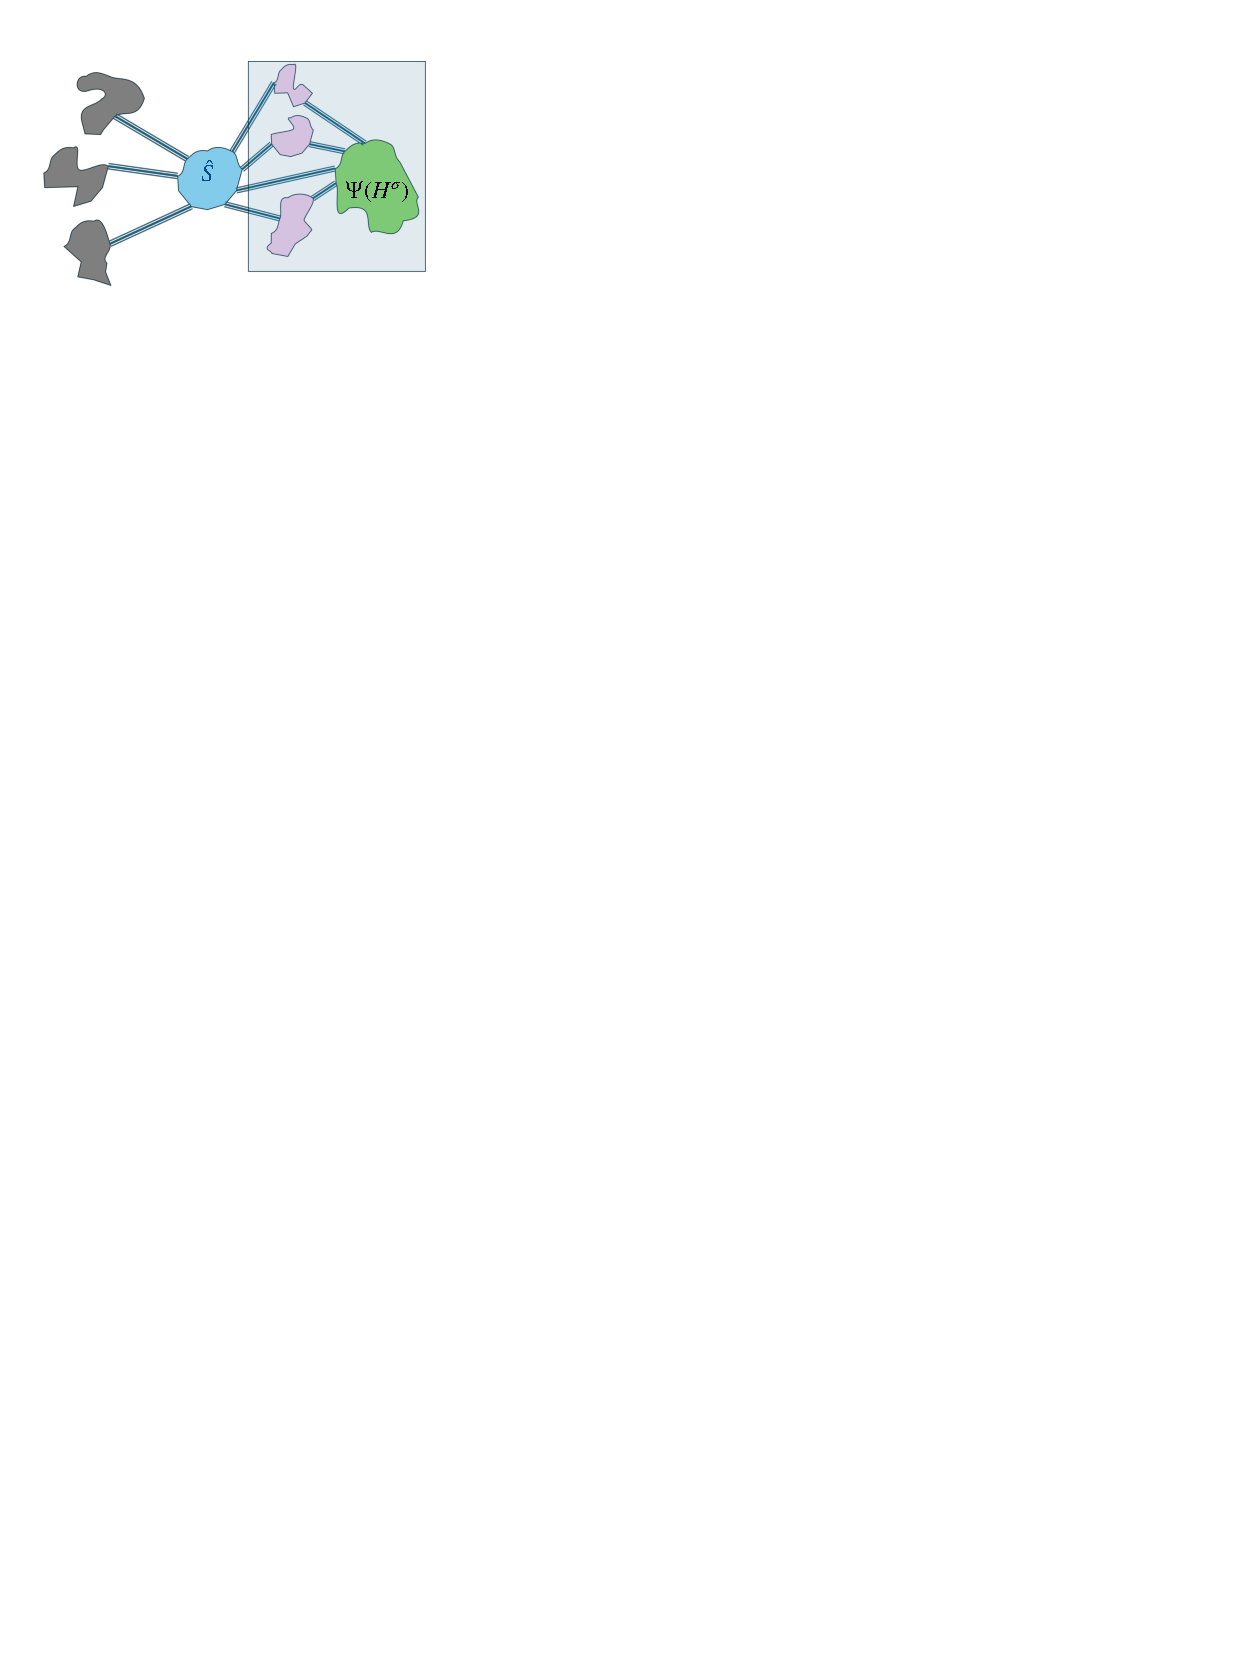
\includegraphics[width=\textwidth]{assets/part-a.pdf}
        \caption{}
    \end{subfigure}
    \hfill
    \begin{subfigure}[t]{0.3\textwidth}
        \centering
        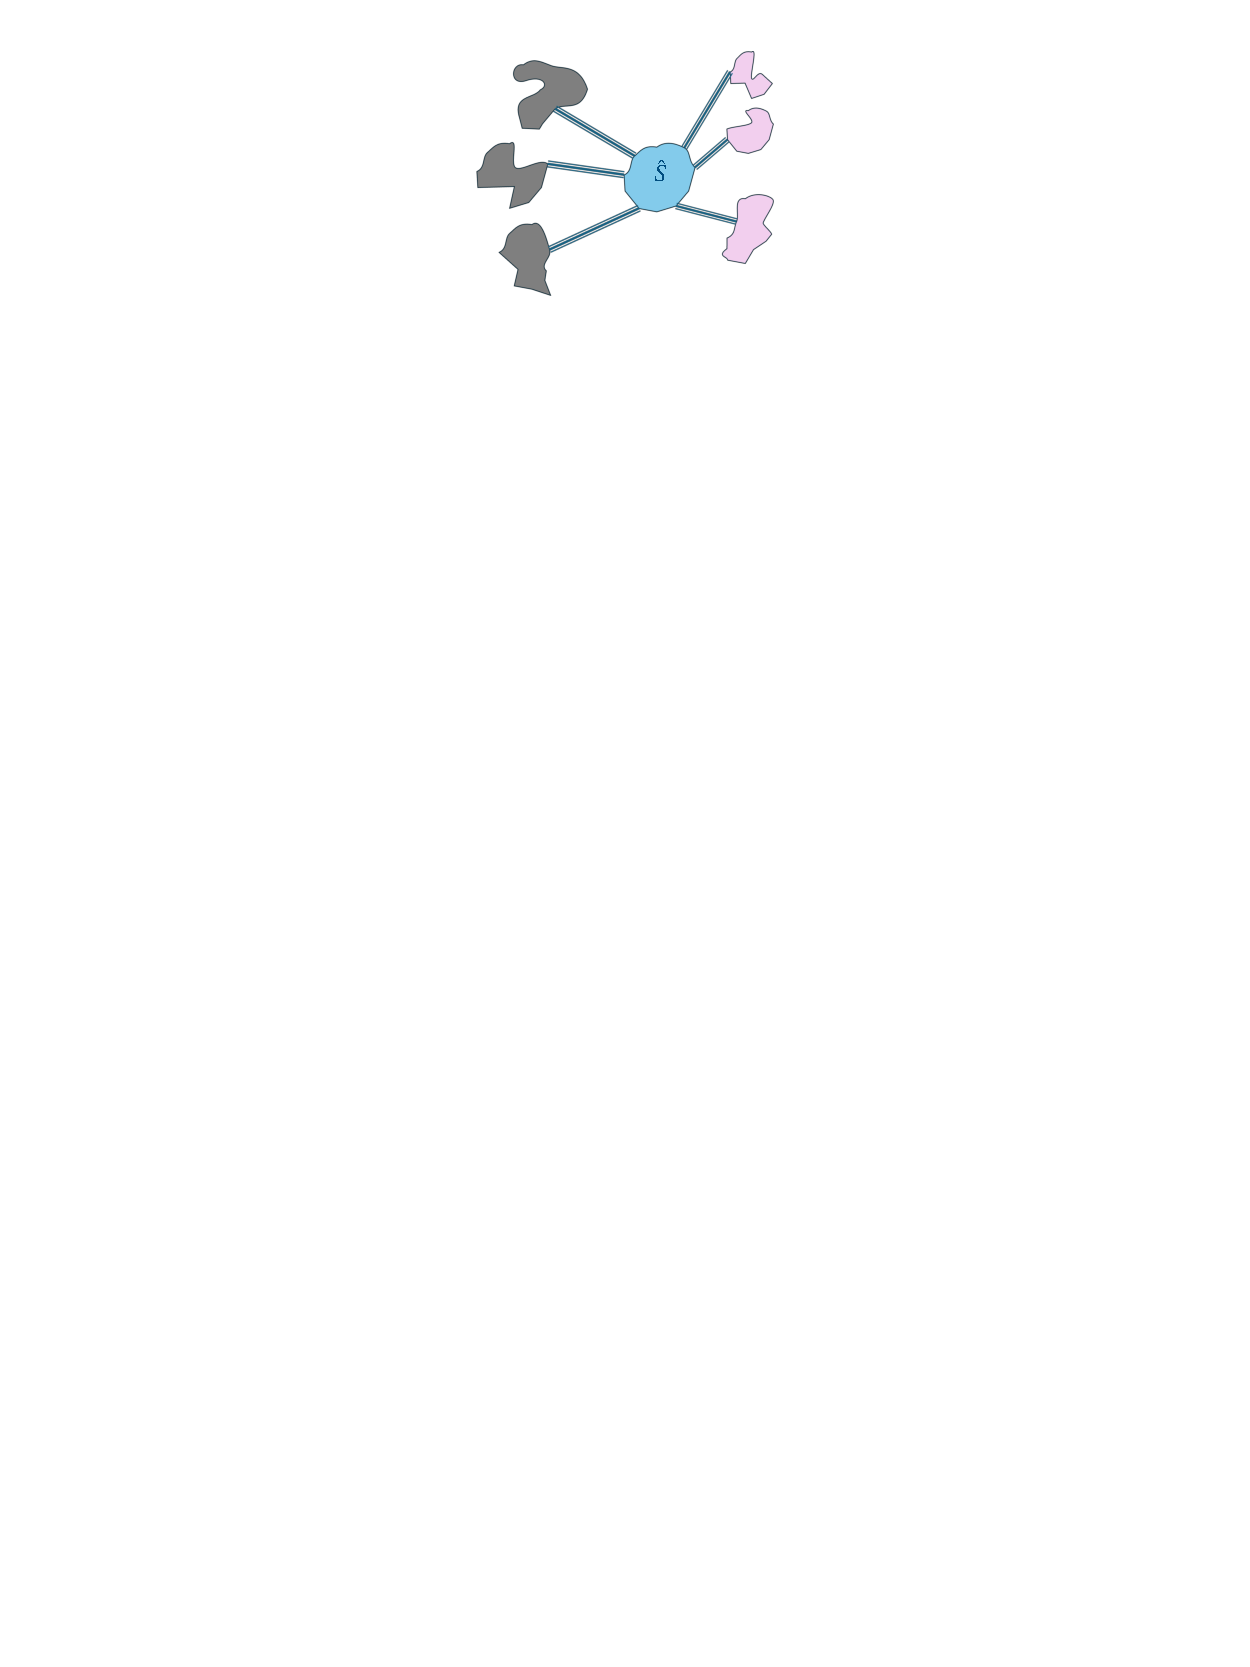
\includegraphics[width=\textwidth]{assets/part-b.pdf}
        \caption{
        }
    \end{subfigure}
    \hfill
    \begin{subfigure}[t]{0.3\textwidth}
        \centering
        
\includegraphics[width=\textwidth]{assets/part-c.pdf}
        \caption{\small Caption for Part C.}
    \end{subfigure}
    \caption{The blue box denotes the single connected component $U$ in $G$, and the grey blobs denote the connected components attached to $\BadSet$ that are unaffected by the deletion of $\Embedding{\Subdivision{H}{\sigma}}$. By our assumption, deleting $\Embedding{\Subdivision{H}{\sigma}}$ from $G$ causes $U$ to split into many components (shown in pink) such that the number of odd sized components exceeeds $\Size{\BadSet}$. By definition, all edges connections between these components should go via $\BadSet$. Thus, on deletion of $\BadSet$ there should be no edge between $X$ and $Y$. We show that one exists, thus our assumption must have been wrong.}
    \label{fig:three-images}
\end{figure*}


\begin{theorem}[Perfect Matching On The Remainder Theorem]\label{thm:perfect-matching}
Given $\EnDeeLambda$ graph $\Graph=(V,E)$, let $\Embedding{\Subdivision{H}{\sigma}}$ be the topological embedding of the hard instance $H$ from Theorem \ref{thm:top-embedding}.
Then the induced sub-graph $\Graph[V \setminus \Embedding{\Subdivision{H}{\sigma}}]$ has a perfect matching.	
	
\end{theorem}



\begin{proof}Let $\RemGraph \Def  \Graph[V \setminus \Embedding{\Subdivision{H}{\sigma}}]$ and $\Size{\Vertices{\RemGraph}}\Def \SizeRemGraph$.
  Let $\RedA$ and $\GreenB$ denote the balanced sets from Theorem \ref{thm:partition}.
  We refer the reader to Remark \ref{remark:edge-dist} for a review of how the many red and green neighbours each vertex in $G$ has.
\textit{\highlight{Assume towards a contradiction} that $\RemGraph$ does \textbf{not} admit a perfect matching.}
By the \nameref{lemma:tutte-criterion}, this implies that there exists a bad set $\BadSet$ such that $\OddComponents{\RemGraph \setminus \BadSet} > |\BadSet|$.
Note that if $\Size{\BadSet} \geq \SizeRemGraph/2$, then by simple counting argument $\OddComponents{\RemGraph \setminus \BadSet} \leq |\BadSet|$ (there are not enough vertices left in $\RemGraph$ to make more than $\SizeRemGraph/2$ connected components).
So we can assume that $\Size{\BadSet} \leq \SizeRemGraph/2$.\\
Now, we know from Lemma \ref{lemma:edge-connectivity-pseudorandom} that $G$ is $d$ edge connected, therefore by Lemma  \ref{lemma:d-connected-sets-have-no-bad-sets} we get that for any set $S \subseteq \Vertices{G}$, we have $\OddComponents{G \setminus S} \leq |S|$.  
Also as $\Embedding{\Subdivision{H}{\sigma}}$ is a connected\footnote{The proof also works if the embedding being removed is not connected, but the presence of connectedness makes the proof simpler to write.} subgraph contained entirely in $\GreenB$, it must be entirely contained in one of the connected components connected to $\BadSet$. Figure \ref{fig:before-deletions} illustrates what we have described above pictorially.
We denote this connected component with $U$.
Now for $\RemGraph$ to \highlight{not} admit a perfect matching, the process of deleting edges incident on $\Embedding{\Subdivision{H}{\sigma}}$ and $\BadSet$ must at some point cause $U$ to split into more than 1 disconnected components, which causes $\OddComponents{\RemGraph \setminus \BadSet}$ to cross over the threshold $|\BadSet|$.
Figure \ref{fig:after-deletions} describes this event.
To arrive at our \textit{\highlight{contradiction}}, we will show that there there \emph{must} be at least one edge between newly formed disconnected components, which contradicts the claim that they are disconnected components, which completes our proof.

Let $X$ and $Y$ denote a partition of $\Vertices{\RemGraph} \setminus \BadSet$ suc that $\Size{X} \geq \Size{\BadSet}/4$ and $\Size{Y} \geq \Size{\BadSet}/4$.
(See Figure \ref{fig:contradiction} for a reference).
This is always possible given $\Size{\BadSet} \leq \SizeRemGraph/2$.
Without loss of generality let $\Size{Y} \leq \Size{X}$.
Then $\Size{Y} < (\SizeRemGraph-|\BadSet|)/2$.
By the balanced partition theorem, every vertex in $Y$ has at least $\frac{11d}{16}$ \red{red} neighbours in $\RemGraph$.
To see why observe that removing $\Embedding{\Subdivision{H}{\sigma}}$ from $G$ does not affect the red edge distribution, as $\Embedding{\Subdivision{H}{\sigma}}$ is composed entirely of \green{green} vertices.
So there \emph{MUST} be at least $\frac{11d}{16}\Size{Y}$ edges incident on $Y$ (where we count edges with both end-points in $Y$ twice).

\begin{equation}\label{eq:edge-lower-bound}
  \CutEdges{Y}{Y}{\Edges{\RemGraph}} \geq \frac{11d}{16}\Size{Y}
\end{equation}

Now by the \nameref{lemma:expanders-mixing-lemma} with relations to edges in the orignal graph $G$,

\begin{align}
  \CutEdges{Y}{Y}{\Edges{G}}  &\leq \frac{d}{n}\Size{Y}^2 + \lambda\Size{Y} \\
  &\leq \frac{d}{\SizeRemGraph}\Size{Y}^2 + \epsilonL d \Size{Y} \label{eq:why}
\end{align}

Where Equation \eqref{eq:why} comes from the fact that $\SizeRemGraph \leq n$ and our spectral assumption that $\lambda \leq \epsilonL d$.
Also by the expander mixing lemma,

\begin{align}
  \CutEdges{\BadSet}{Y}{\Edges{G}}  &\leq \frac{d}{n}\Size{\BadSet}\Size{Y} + \lambda\sqrt{\Size{Y}\Size{\BadSet}} \\
                                    &\leq \frac{d}{\SizeRemGraph}\Size{\BadSet}\Size{Y} + \epsilonL d\sqrt{\Size{Y}\Size{\BadSet}} \\
  &\leq \frac{d}{\SizeRemGraph}\Size{\BadSet}\Size{Y} + 2\epsilonL d\Size{Y} \label{eq:why2}
\end{align}

Step \eqref{eq:why2} comes from the assumption that $\Size{\BadSet} \leq 4\Size{Y}$. Combining equations \eqref{eq:why} and \eqref{eq:why2}, gives us the total number of edges incident on $Y$ either from $\BadSet$ or edges incident from $Y$ itself (i.e these edges have both endpoints in $Y$) is $\frac{d}{\SizeRemGraph}\Size{Y}^2 +   \frac{d}{\SizeRemGraph}\Size{\BadSet}\Size{Y} + 3\epsilonL d\Size{Y}$.

\begin{align}
 \text{Total edges in $\RemGraph$ incident on $Y$ from $\BadSet$ and $Y$} &\leq \frac{d\Size{Y}^2}{\SizeRemGraph} +   \frac{d}{\SizeRemGraph}\Size{\BadSet}\Size{Y} + 3\epsilonL d\Size{Y}\\[3pt]                                                                          &\leq  \frac{d\Size{Y}}{\SizeRemGraph}\frac{(\SizeRemGraph - \Size{\BadSet})}{2} + \frac{d}{\SizeRemGraph}\Size{\BadSet}\Size{Y} + 3\epsilonL d\Size{Y} \label{eq:why3}\\[3pt]
                                                                          &= \frac{d\Size{Y}}{2} + \frac{d\Size{\BadSet}\Size{Y}}{2\SizeRemGraph} +3\epsilonL d\Size{Y}\\[3pt]
                                                                          &\leq \frac{d\Size{Y}}{2} + \frac{d\Size{Y}}{4} +3\epsilonL d\Size{Y}  \label{eq:why4}\\
                                                                            &< \frac{11d}{16}\Size{Y} \label{eq:edge-upperbound}
\end{align}

Equation \eqref{eq:why3} comes from  $\Size{Y} < (\SizeRemGraph - \Size{\BadSet})/2$.
Equation \eqref{eq:why4} comes from the assumption that $\Size{\BadSet} \leq \SizeRemGraph/2$.
The lower bound on the edges incident on $Y$ given in Equation \eqref{eq:edge-lower-bound} strictly greater than the upper bound in Equation \eqref{eq:edge-upperbound}.
This implies that there \emph{must} be edges incident on $Y$ from sets that are neither $Y$ or $\BadSet$.
Therefore, there must be an edge from $X$ into $Y$.
This means $X$ and $Y$ cannot be disconnected as we \highlight{assumed}.
We have our contradiction.

\end{proof}

\section{Related Work}
\label{sec:related-work}




\bibliographystyle{unsrtnat}
\bibliography{main_paper}
\clearpage
\appendix
\section{Extra Stuff TO SORT OUT later}
\subsection{Graph Theory Preliminaries}

% $\CutEdgesSet{S_k}{S_k'}{E_{\GreenB}}$ define\todo{do}

% \begin{definition}[Subgraph]\label{def:subgraph}
% A graph $G'=(V', E')$ is a subgraph of another graph $G=(V, E)$ iff (1) $V'\subseteq V$, and (2) $E'\subseteq E$ and  $(v_1, v_2) \in E' \implies (v_1, v_2) \in V')$.
	
% \end{definition}



\end{document}
